% !TeX root = statnicaEKT.tex
\graphicspath{{Obrazky/Obrazky_NEZ/}}
\part{BPC-NEZ - Návrh elektronických zařízení}
\begin{huge}
	Otázky:
	\newline
\end{huge}
\begin{enumerate}
	\item Transformátory a tlumivky pro napájecí zdroje, princip, návrh, materiály jádra, vodiče pro vinutí, parazitní vlastnosti.
	\item Neřízené usměrňovače, zapojení, dimenzování prvků, vliv reálných vlastností komponent, napěťové násobiče.
	\item Referenční zdroje napětí, principy, požadavky, teplotní kompenzace.
	\item Spojité parametrické stabilizátory: princip, návrh, vlastnosti.
	\item Spojité lineární stabilizátory, zapojení, stabilita, vlastnosti integrovaných verzí.
	\item Spínané měniče s galvanickou vazbou, princip, zapojení silových obvodů, nábojové pumpy.
	\item Spínané měniče s transformátorem, princip, zapojení silových obvodů, vlastnosti.
	\item Můstkové měniče, princip, zapojení silových obvodů, vlastnosti.
	\item Elektrochemické zdroje proudu, chlazení součástek, přepěťové a nadproudové jištění napájecích zdrojů, korektory účiníku.
	\item Parametry výkonových tranzistorů z hlediska napájecích zdrojů, přechodové jevy při spínání a vypínání indukčních zátěží a jejich potlačení.
\end{enumerate}
%%%%%%%%%%%%%%%%%%%%%%%%%%%%%%%%%%%%%%%%%%%%%%%%%%%
\chapter{Transformátory a tlumivky pre napájacie zdroje}
%%%%%%%%%%%%%%%%%%%%%%%%%%%%%%%%%%%%%%%%%%%%%%%%%%%

\textit{Okruh: Transformátory a tlumivky pro napájecí zdroje, princip, návrh, materiály jádra, vodiče pro vinutí, parazitní vlastnosti.}

\section{Čo je transformátor a na čo slúži?}

Transformátor prenáša elektrickú energiu medzi dvoma obvodmi \textbf{bez priameho elektrického spojenia} -- cez magnetické pole v jadre. Pri tom môže meniť napätie (napr. zo 230~V sieťových na 12~V pre elektroniku). V spínaných zdrojoch slúži aj ako \textbf{galvanická izolácia} -- výstup je bezpečne oddelený od vstupu.

Základný princíp: striedavý prúd v primárnom vinutí ($N_1$ závitov) vytvára v jadre magnetický tok $\Phi$, ktorý indukuje napätie v sekundárnom vinutí ($N_2$ závitov). Pomer napätí sa rovná pomeru počtu závitov:
\[ \frac{u_1}{u_2} = \frac{N_1}{N_2} \]
Ak má primár 100 závitov a sekundár 10 závitov, výstupné napätie bude desaťkrát menšie. Výstupný prúd bude naopak desaťkrát väčší -- výkon sa zachováva (za predpokladu nulovej straty).

\textbf{Dôležité obmedzenie:} primárne napätie musí mať \textbf{nulovú strednú hodnotu} (musí byť striedavé). Ak by sme priložili jednosmerné napätie, magnetizačný prúd by rástol bez obmedzenia, jadro by sa nasýtilo a transformátor by prestal fungovať -- zvyčajne by sa pritom zničil.

\section{Tri modely transformátora}

V praxi sa rozlišujú tri úrovne popisu:
\begin{itemize}
    \item \textbf{Ideálny} -- nekonečné indukčnosti $L_1$ a $L_2$, dokonalá magnetická väzba, bez strát. Používa sa pre základné výpočty prevodového pomeru.
    \item \textbf{Dokonalý} -- konečné indukčnosti $L_1$ a $L_2$, stále dokonalá väzba, stále bez strát. Zahrňuje magnetizačný prúd.
    \item \textbf{Reálny} -- konečné indukčnosti, nedokonalá väzba (rozptylová indukčnosť), straty vo vinutí aj v jadre.
\end{itemize}

\begin{figure}[H]
  \centering
  \begin{subfigure}{0.48\textwidth}
    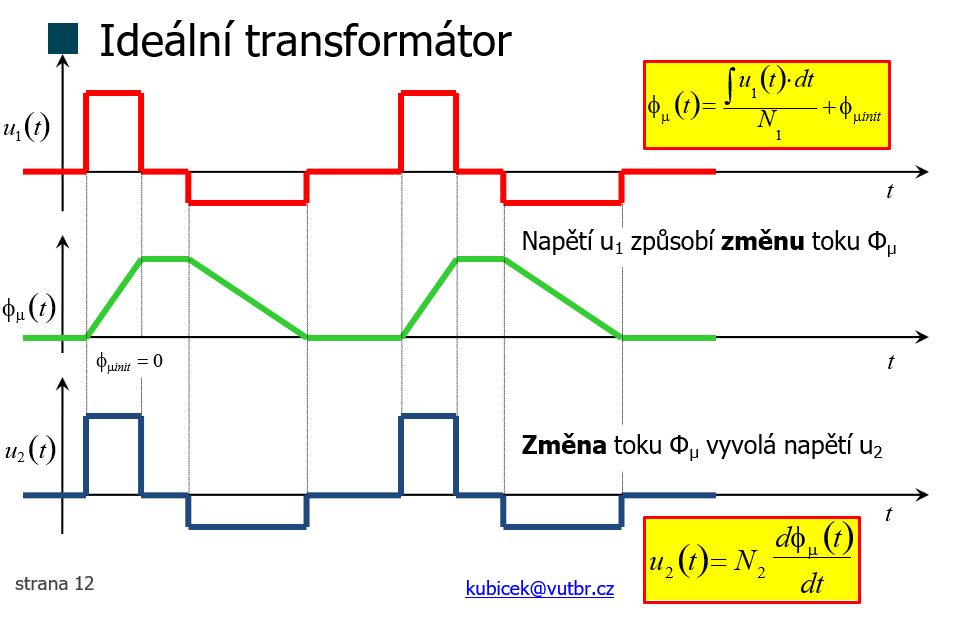
\includegraphics[width=\textwidth]{img_07_idealni_trafo.png}
    \caption{Schéma ideálneho transformátora}
  \end{subfigure}
  \hfill
  \begin{subfigure}{0.48\textwidth}
    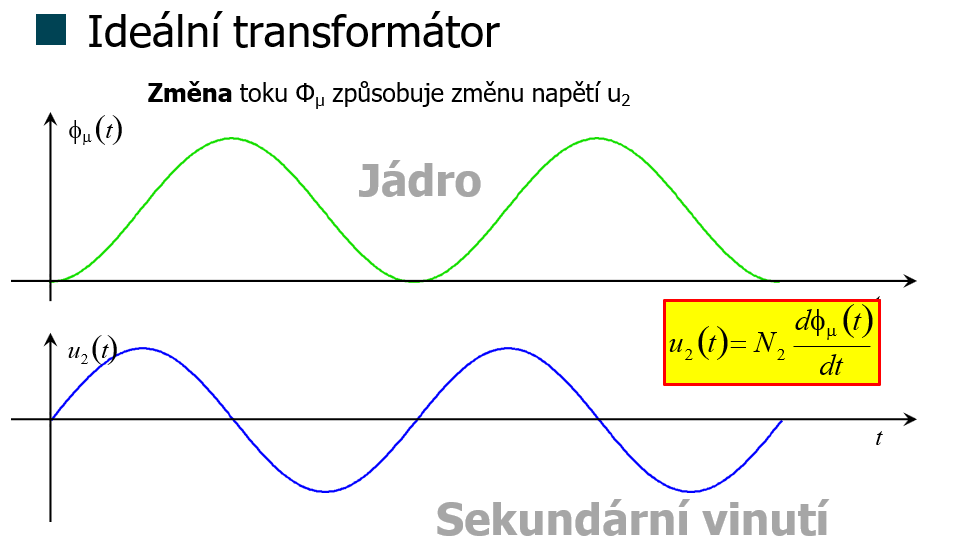
\includegraphics[width=\textwidth]{img_07_idealni_trafo_priebeh.png}
    \caption{Priebeh $u_1$, toku $\Phi$ a $u_2$}
  \end{subfigure}
  \caption{Ideálny transformátor (Prednáška 7, Slide 9 a 11)}
  \label{fig:idealni_trafo}
\end{figure}

\section{Straty v reálnom transformátore}

Existujú štyri hlavné zdroje strát:

\begin{itemize}
    \item \textbf{Jouleove straty vo vinutí} -- vodič má odpor, prúd ho ohrieva ($P = R \cdot I^2$). Pri vyšších frekvenciách nastáva \textit{skinefekt}: prúd tečie len po povrchu vodiča, efektívny odpor rastie s frekvenciou. Navyše \textit{jav blízkosti} (proximity effect) -- susedné vodiče ovplyvňujú rozloženie prúdu. Preto sa pri impulzných transformátoroch používa \textbf{lankový vodič} (litz wire) -- veľa tenkých izolovaných vlákien namiesto jedného hrubého.
    \item \textbf{Hysterézne straty v jadre} -- feromagnetické jadro sa pri každej perióde premagnetuje pozdĺž hysteréznej slučky -- to stojí energiu. Tieto straty rastú \textit{priamo úmerne} s frekvenciou ($P_h \propto f$).
    \item \textbf{Straty vírivými prúdmi v jadre} -- meniaci sa magnetický tok indukuje v vodivom jadre vírivé prúdy, ktoré ho ohrievajú. Rastú so \textit{štvorcom frekvencie} ($P_v \propto f^2$). Znižujú sa použitím izolovaných plátkov (transformátorové plechy) alebo feritových jadier, ktoré elektricky nevedú.
    \item \textbf{Rozptylová indukčnosť} -- nie všetok magnetický tok prechádza cez obe vinutia, časť ``unikne'' do okolia. Tento rozptyl sa modeluje sériovou rozptylovou indukčnosťou $L_R$, ktorá spôsobuje napäťový úbytok a nebezpečné napäťové špičky pri vypínaní spínača v impulzných obvodoch.
\end{itemize}

\begin{figure}[H]
  \centering
  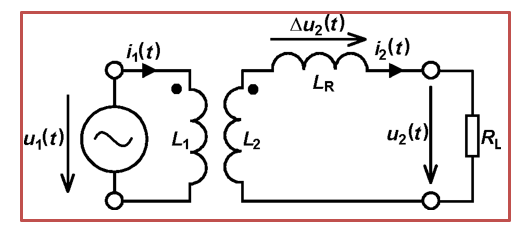
\includegraphics[width=0.70\textwidth]{img_07_realni_trafo_model.png}
  \caption{Náhradný obvod reálneho transformátora -- odpory vinutí $R_1, R_2$, rozptylová indukčnosť $L_R$ a magnetizačná indukčnosť $L_\mu$ (Prednáška 7, Slide 40)}
  \label{fig:realni_trafo}
\end{figure}

\section{Materiály jadier}

Voľba materiálu závisí predovšetkým od pracovnej frekvencie a požadovanej maximálnej indukcii $B_M$:

\begin{center}
\begin{tabular}{llll}
\toprule
\textbf{Materiál} & \textbf{Frekvencia} & \textbf{$B_M$} & \textbf{Typické použitie} \\
\midrule
Elektrotechnické plechy (Si) & 50~Hz -- 400~Hz & až 1,6~T & Sieťové transformátory \\
Ferity & 10~kHz -- 10~MHz & až 0,5~T & Impulzné transformátory, tlumivky \\
Amorfné materiály & do MHz & 1--1,5~T & Výkonové impulzné zdroje \\
\bottomrule
\end{tabular}
\end{center}

\textbf{Ferity} sú keramické materiály -- elektricky nevedú, takže v nich nevznikajú vírivé prúdy. Preto sú ideálne pre vysoké frekvencie spínaných zdrojov. Nevýhoda: nižšia sýtacia indukcia (0,3--0,5~T) oproti plechom (až 1,6~T).

Bežné tvary jadier: \textbf{E-E, ETD, RM, hrníčkové (pot core), toroidné, planárne}. Impulzné transformátory najčastejšie používajú tvary ETD alebo E-E.

\begin{figure}[H]
  \centering
  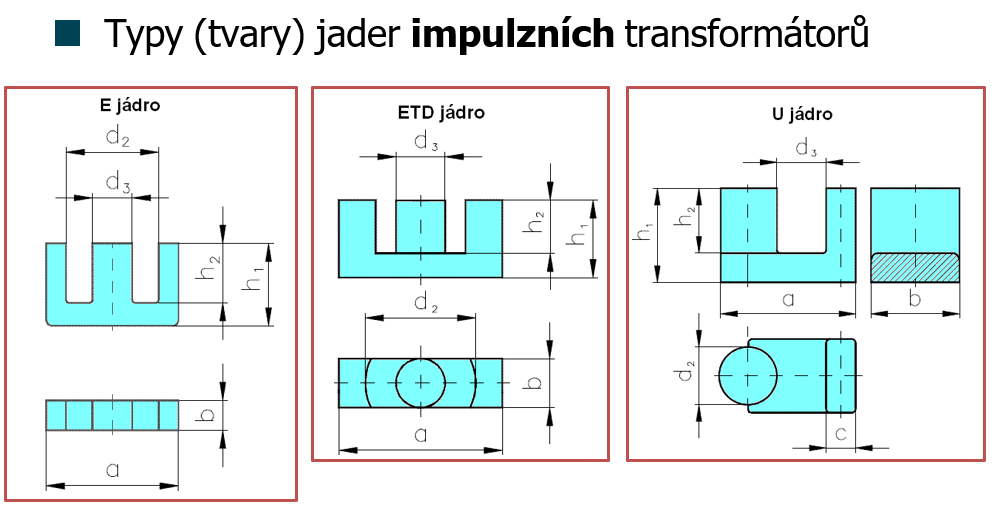
\includegraphics[width=0.75\textwidth]{img_07_typy_jader.png}
  \caption{Typy jadier impulzných transformátorov -- E-E, ETD, hrníčkové, toroidné, planárne (Prednáška 7, Slide 58)}
  \label{fig:typy_jader}
\end{figure}

\section{Vodiče pre vinutie}

Maximálna prúdová hustota závisí od podmienok chladenia:
\begin{itemize}[noitemsep]
    \item Vodiče vo voľnom priestore: až 15~A/mm²
    \item Vinutia malých transformátorov: až 6~A/mm²
    \item Vinutia väčších transformátorov: 2--4~A/mm²
\end{itemize}
Pre zníženie skinefektu pri vysokých frekvenciách sa používa lankový vodič (litz wire). Pre planárne transformátory sa vinutie realizuje priamo ako meď na plošnom spoji (PCB winding).

\section{Tlumivka -- akumulátor energie}

Tlumivka (cívka s jadrom) slúži v DC/DC meniačoch ako \textbf{akumulátor energie} -- keď spínač sepne, ukladá energiu do magnetického poľa; keď spínač rozopne, uvoľní energiu do záťaže a vyhladzuje prúd.

Na rozdiel od transformátora je tlumivka \textbf{budená prúdom} (nie napätím). Aby sa jadro nenasýtilo pri veľkých prúdoch, zaraďuje sa do magnetického obvodu \textbf{vzduchová medzera}. Väčšina energie sa sústredí práve v tejto medzere (vzduch má oveľa menšiu permeabilitu ako ferit), čo umožňuje dosiahnuť potrebnú indukčnosť bez nasýtenia jadra.

\begin{figure}[H]
  \centering
  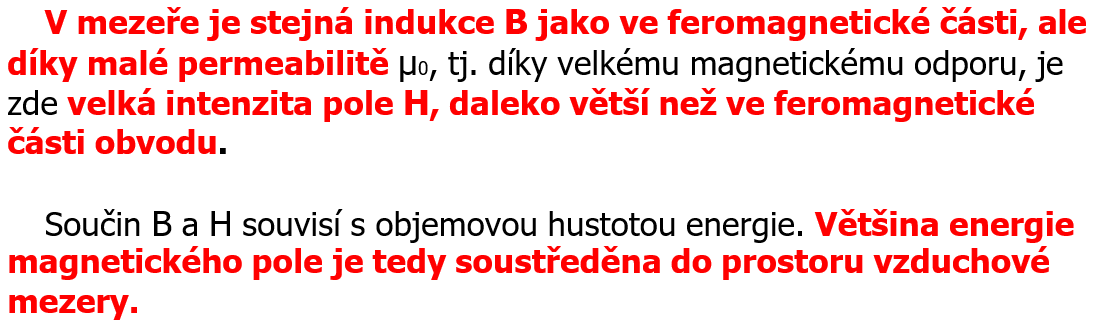
\includegraphics[width=0.55\textwidth]{img_07_tlumivka_mezera.png}
  \caption{Tlumivka s vzduchovou medzerou -- väčšina energie je sústredená v medzere (Prednáška 7, Slide 78)}
  \label{fig:tlumivka_mezera}
\end{figure}

Pre tlumivky v spínaných zdrojoch sa využívajú aj \textbf{prášková jadrá} (Sendust, MPP, KoolMu, XFlux) -- vzduchová medzera je rozložená rovnomerne v celom objeme materiálu. To umožňuje väčší prúdový rozkmit bez ostrého nasýtenia.

%%%%%%%%%%%%%%%%%%%%%%%%%%%%%%%%%%%%%%%%%%%%%%%%%%%
\chapter{Neřízené usměrňovače}
%%%%%%%%%%%%%%%%%%%%%%%%%%%%%%%%%%%%%%%%%%%%%%%%%%%

\textit{Okruh: Neřízené usměrňovače, zapojení, dimenzování prvků, vliv reálných vlastností komponent, napěťové násobiče.}

\section{Čo robí usmerňovač?}

Usmerňovač mení striedavé napätie (zo siete alebo z transformátora) na jednosmerné. Robí to pomocou diód -- tie prepúšťajú prúd len jedným smerom. Výsledok nie je ideálne rovné jednosmerné napätie, ale \textbf{pulzujúce} -- preto sa za usmerňovač zaraďuje filtračný kondenzátor, ktorý zvlnenie vyhladí.

\section{Typy zapojení}

\subsection{Jednopolcestný usmerňovač}

Najjednoduchší -- jedna dióda. Prepúšťa len kladné polperiódy, záporné odreže. Stredná hodnota výstupného napätia je $U_0 \approx 0{,}318 \cdot U_{2\max}$ -- teda len asi tretina maximálneho napätia. Zvlnenie je veľké a transformátor je jednosmernou magnetizáciou nerovnomerne zaťažený. Používa sa len v najjednoduchších prípadoch.

\begin{figure}[H]
  \centering
  \begin{subfigure}{0.48\textwidth}
    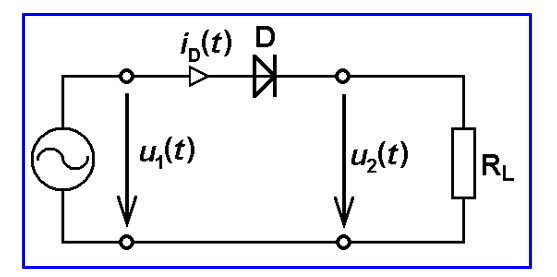
\includegraphics[width=\textwidth]{img_06_jednocestny.png}
    \caption{Schéma zapojenia}
  \end{subfigure}
  \hfill
  \begin{subfigure}{0.48\textwidth}
    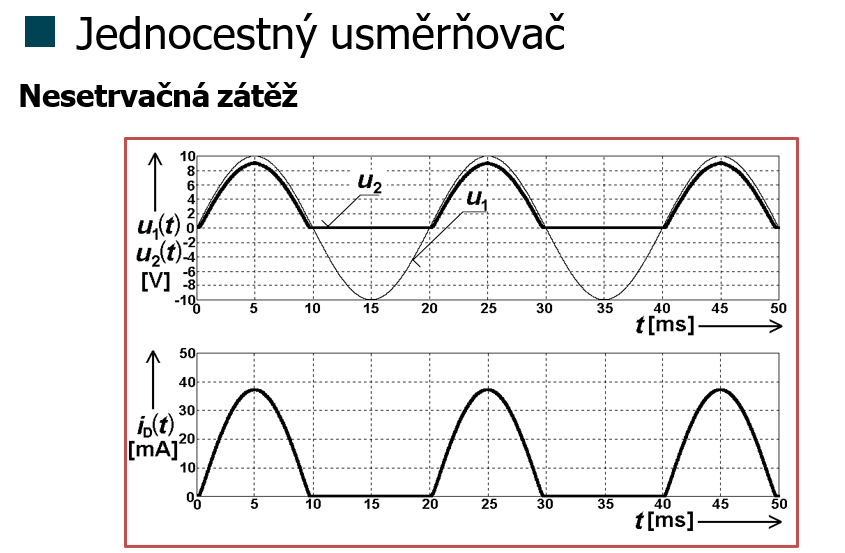
\includegraphics[width=\textwidth]{img_06_jednocestny_priebeh.png}
    \caption{Priebeh napätia na výstupe}
  \end{subfigure}
  \caption{Jednopolcestný usmerňovač (Prednáška 6, Slide 100 a 101)}
  \label{fig:jednocestny}
\end{figure}

\subsection{Grätzov mostíkový usmerňovač}

Štyri diódy v mostíkovom zapojení -- \textbf{najpoužívanejší typ}. Využíva obe polperiódy: v kladnej polperióde vedú dve diódy, v zápornej druhé dve. Výsledok: výstupné napätie pulzuje s dvojnásobnou frekvenciou (pri 50~Hz sieťovom napätí 100-krát za sekundu), zvlnenie je menšie a stredná hodnota napätia je $U_0 \approx 0{,}637 \cdot U_{2\max}$. Na každej dióde je maximálne závěrné napätie rovné $U_{2\max}$.

\begin{figure}[H]
  \centering
  \begin{subfigure}{0.48\textwidth}
    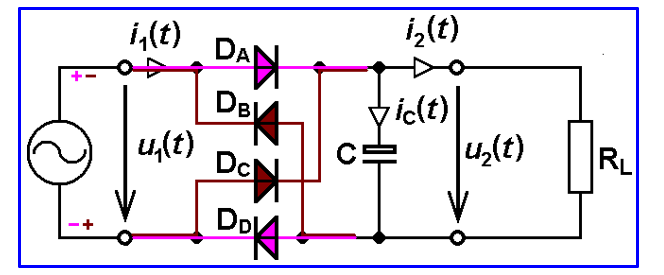
\includegraphics[width=\textwidth]{img_06_graetz.png}
    \caption{Schéma mostíkového usmerňovača}
  \end{subfigure}
  \hfill
  \begin{subfigure}{0.48\textwidth}
    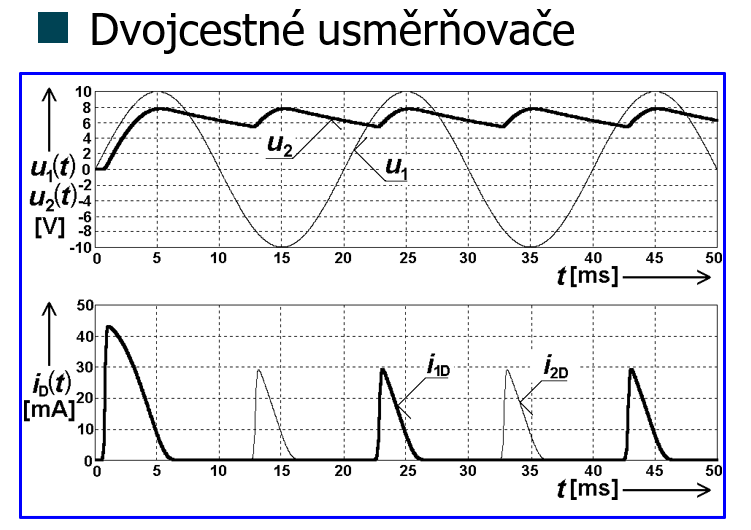
\includegraphics[width=\textwidth]{img_06_graetz_priebeh.png}
    \caption{Priebeh výstupného napätia}
  \end{subfigure}
  \caption{Grätzov mostíkový usmerňovač (Prednáška 6, Slide 110 a 111)}
  \label{fig:graetz}
\end{figure}

\section{Dimenzovanie prvkov}

Pri výbere diód treba zohľadniť:
\begin{itemize}
    \item \textbf{Závěrné napätie} ($U_{RRM}$) -- maximálne napätie, ktoré dióda vydrží v závernom smere. Musí byť s rezervou (typicky $1{,}5\times$) vyššie ako maximálne napätie v obvode.
    \item \textbf{Stredný priamy prúd} ($I_{F,AV}$) -- priemerný prúd prechádzajúci diódou.
    \item \textbf{Neopakovateľný špičkový prúd} ($I_{FSM}$) -- pri zapnutí zdroja sa nenabité kondenzátory správajú ako skrat a tečie krátky veľký prúd; dióda to musí vydržať.
    \item \textbf{Vypínacia doba} ($t_{rr}$) -- dôležitá pre spínané zdroje; pomalá dióda sa stáva zdrojom strát.
\end{itemize}

\textbf{Typy diód:}
\begin{itemize}
    \item \textbf{Bežné kremíkové (Si)} -- veľké závěrné napätie, úbytok $\approx 0{,}7$~V, pomalé -- vhodné pre sieťové frekvencie.
    \item \textbf{Schottkyho} -- malý úbytok ($\approx 0{,}3$~V), veľmi rýchle, ale max. závěrné napätie len $\approx 60$~V. Ideálne pre nízkoapäťové výstupy spínaných zdrojov.
    \item \textbf{Fast Recovery} -- kremík so skrátenou dobou $t_{rr}$, pre stredné frekvencie (desiatky kHz).
\end{itemize}

\textbf{Vplyv reálnych vlastností:} Reálny elektrolytický kondenzátor má \textbf{ESR} (ekvivalentný sériový odpor). Pri veľkých nabíjacích prúdových pulzoch spôsobuje ESR dodatočné zvlnenie výstupného napätia a ohrev kondenzátora -- to je dôležitý limitujúci faktor pri voľbe kondenzátora pre spínané zdroje.

\section{Napäťové násobiče}

Niekedy potrebujeme vysoké napätie, ale bez výkonového transformátora. Riešenie: \textbf{Greinacherov zdvojovač} -- dve diódy a dva kondenzátory. Počas jednej polperiódy sa nabije jeden kondenzátor, počas druhej druhý, a na výstupe sa napätia sčítajú -- výsledok je $\approx 2 \cdot U_{2\max}$.

Kaskádovým zapojením viacerých stupňov (\textbf{Delonov násobič}) možno dosiahnuť $n \cdot U_{2\max}$, kde $n$ je počet stupňov. Za cenu rastúceho zvlnenia a úbytku napätia pri zaťažení. Vhodné pre CRT monitory, elektrostatiku a vysokonapäťové aplikácie s malým odberom.

\begin{figure}[H]
  \centering
  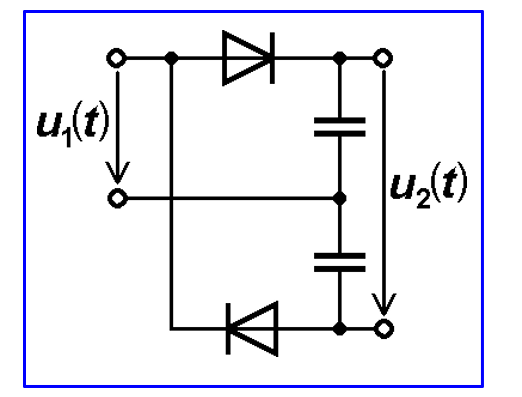
\includegraphics[width=0.65\textwidth]{img_06_nasobic.png}
  \caption{Greinacherov zdvojovač napätia a Delonov násobič (Prednáška 6, Slide 116--117)}
  \label{fig:nasobic}
\end{figure}

%%%%%%%%%%%%%%%%%%%%%%%%%%%%%%%%%%%%%%%%%%%%%%%%%%%
\chapter{Referenčné zdroje napätia}
%%%%%%%%%%%%%%%%%%%%%%%%%%%%%%%%%%%%%%%%%%%%%%%%%%%

\textit{Okruh: Referenční zdroje napětí, principy, požadavky, teplotní kompenzace.}

\section{Prečo potrebujeme referenciu?}

Každý spätnoväzbový stabilizátor porovnáva výstupné napätie s \textbf{referenčným napätím}. Ak je referencia nepresná alebo sa mení s teplotou, mení sa aj výstupné napätie celého zdroja. Preto sú na referenčný zdroj kladené tieto požiadavky:
\begin{itemize}[noitemsep]
    \item Malá tolerancia napätia ($\pm 0{,}1$\,\% a lepšie)
    \item Malý teplotný koeficient (TC) -- výstupné napätie sa nesmie meniť s teplotou
    \item Dlhodobá stabilita (stárnutie)
    \item Nízky šum
    \item Malý výstupný odpor
\end{itemize}

\section{Zenerova dióda ako referencia}

Zenerova dióda v závernom smere nastane priepaz pri definovanom napätí $U_Z$ a udržuje ho relatívne stabilne bez ohľadu na prúd. Dynamický odpor $r_Z$ je malý (jednotky až desiatky $\Omega$) -- to zabezpečuje stabilizáciu.

\textbf{Teplotné správanie} závisí od mechanizmu priepazu:
\begin{itemize}
    \item Pod $\approx 6$~V prevláda \textbf{Zenerov (tunelový) jav} -- napätie s teplotou \textit{klesá} (záporný TC).
    \item Nad $\approx 6$~V prevláda \textbf{lavinový priepaz} -- napätie s teplotou \textit{rastie} (kladný TC).
    \item Okolo 6~V sa oba efekty navzájom rušia -- teplotný koeficient $TC \approx 0$.
\end{itemize}

\textbf{Teplotná kompenzácia:} Ak chceme použiť Zenerovu diódu s iným napätím ($\neq 6$~V), môžeme sériovo zaradiť kremíkový PN prechod v priepustnom smere. Ten má záporný $TC \approx -2{,}3$~mV/K a kompenzuje kladný koeficient Zenerovej diódy s vyšším $U_Z$.

\begin{figure}[H]
  \centering
  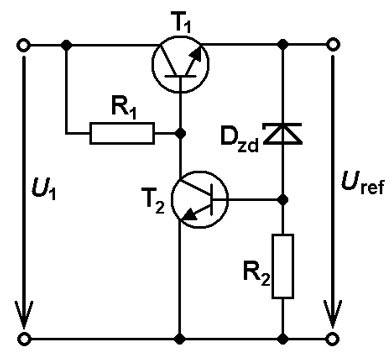
\includegraphics[width=0.60\textwidth]{img_03_zener_kompenzace.png}
  \caption{Teplotne kompenzovaná referencia -- Zenerova dióda v sérii s priepustným prechodom BE tranzistora $T_2$ (Prednáška 3, Slide 27)}
  \label{fig:zener_komp}
\end{figure}

\textbf{Termostatovanie:} najlepší spôsob -- referenčná dióda je udržiavaná na konštantnej teplote ($\approx 90$~°C) pomocou zabudovaného vykurovacieho obvodu. Príklad: LM199 s $TC = 0{,}0001$\,\%/°C.

\section{Band-Gap referencia}

Modernejší a presnejší princíp využívaný vo väčšine integrovaných obvodov. Využíva dve vlastnosti PN prechodu kremíka:
\begin{itemize}
    \item Napätie $U_{BE}$ klesá s teplotou: $\frac{dU_{BE}}{dT} \approx -2{,}3$~mV/K (záporný TC).
    \item Rozdiel napätí dvoch tranzistorov pracujúcich pri rôznych prúdových hustotách ($\Delta U_{BE}$) má \textbf{kladný TC} úmerný absolútnej teplote.
\end{itemize}

Správnou kombináciou (zosilnením $\Delta U_{BE}$ a sčítaním s $U_{BE}$) sa oba TC navzájom presne vyrušia. Výsledné referenčné napätie je $U_{ref} \approx 1{,}25$~V -- táto hodnota súvisí so šírkou zakázaného pásu (band-gap) kremíka ($E_g \approx 1{,}25$~eV) extrapolovanou na 0~K.

\begin{figure}[H]
  \centering
  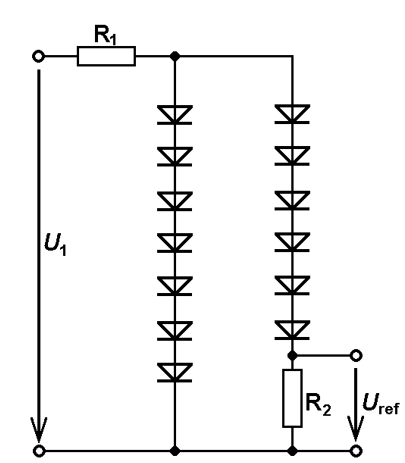
\includegraphics[width=0.65\textwidth]{img_03_bandgap.png}
  \caption{Princíp band-gap referencie -- kompenzácia záporného TC napätia $U_{BE}$ kladným TC rozdielu $\Delta U_{BE}$ (Prednáška 3, Slide 32)}
  \label{fig:bandgap}
\end{figure}


Konkrétne zapojenie \textbf{Brokawovho Band-Gap obvodu} využíva dva tranzistory s rôznymi plochami BE prechodov. Rozdiel ich $U_{BE}$ hodnôt je zosilnený a sčítaný s $U_{BE}$, čím sa navzájom zrušia teplotné koeficienty:

\begin{figure}[H]
  \centering
  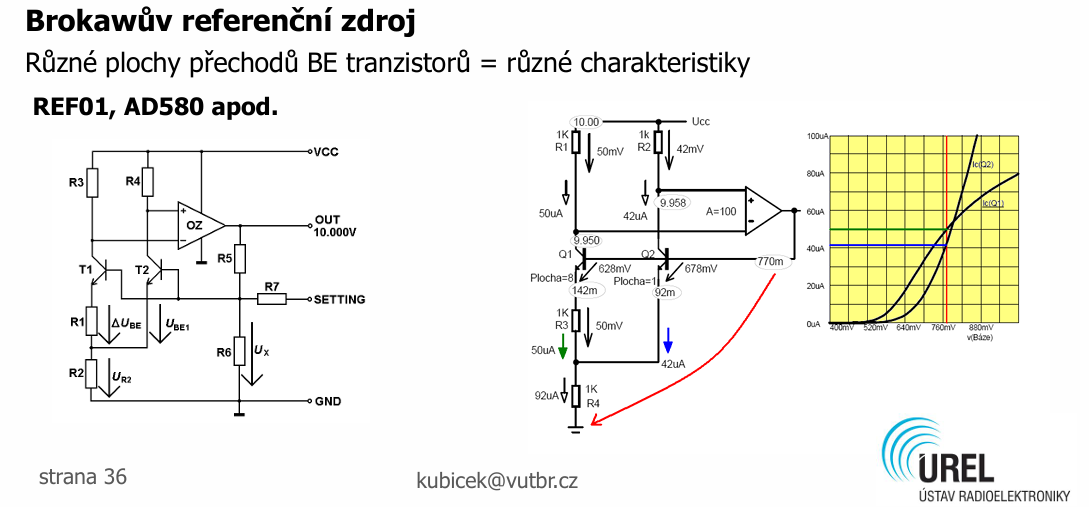
\includegraphics[width=0.55\textwidth]{img_03_brokaw_bg.png}
  \caption{Brokawov Band-Gap referenčný obvod -- dva tranzistory s rôznymi plochami BE prechodov (Prednáška 3, Slide 36)}
  \label{fig:brokaw}
\end{figure}

\textbf{TL431} je integrovaná nastaviteľná napäťová referencia. Operačný zosilňovač vnútri nastavuje prúd diódou presne podľa napätia na REF vstupe:

\begin{figure}[H]
  \centering
  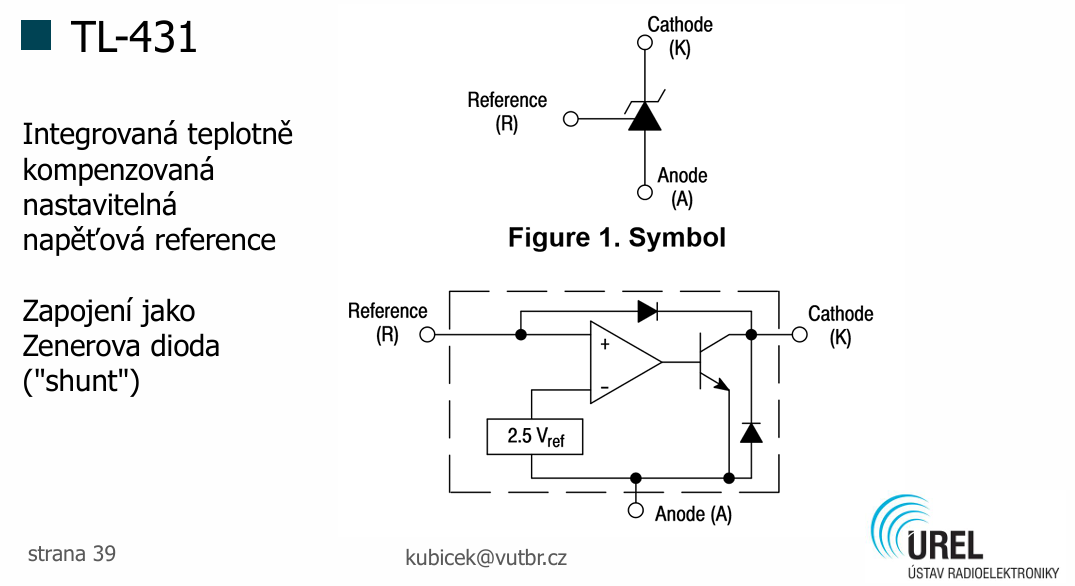
\includegraphics[width=0.55\textwidth]{img_03_tl431.png}
  \caption{TL431 -- základné zapojenie ako nastaviteľná napäťová referencia (Prednáška 3, Slide 39)}
  \label{fig:tl431}
\end{figure}

\textbf{Príklady integrovaných referencií:} TL431 (nastaviteľná 2,5--36~V), LM385 (1,2~V alebo 2,5~V), LM336. Band-gap referencia je zabudovaná aj vo väčšine integrovaných stabilizátorov (78xx, LM317 a ďalších).

%%%%%%%%%%%%%%%%%%%%%%%%%%%%%%%%%%%%%%%%%%%%%%%%%%%
\chapter{Spojité parametrické stabilizátory}
%%%%%%%%%%%%%%%%%%%%%%%%%%%%%%%%%%%%%%%%%%%%%%%%%%%

\textit{Okruh: Spojité parametrické stabilizátory: princip, návrh, vlastnosti.}

\section{Princíp -- regulácia bez spätnej väzby}

Parametrický stabilizátor je najjednoduchší spôsob stabilizácie napätia -- \textbf{žiadna spätná väzba, žiadny zosilňovač}. Funguje vďaka tomu, že Zenerova dióda v oblasti priepazu má veľmi malý \textbf{dynamický odpor} $r_Z$ -- malá zmena napätia spôsobí veľkú zmenu prúdu. Tým absorbuje kolísanie vstupného napätia alebo záťaže.

Zapojenie: sériový odpor $R$ + Zenerova dióda paralelne k záťaži $R_Z$. Odpor $R$ absorbuje rozdiel vstupného a výstupného napätia, Zenerova dióda udržuje výstup stabilný.

\begin{figure}[H]
  \centering
  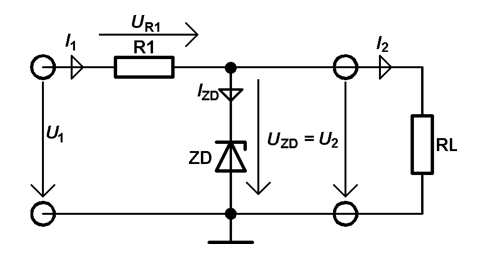
\includegraphics[width=0.55\textwidth]{img_02_param_stabilizator.png}
  \caption{Parametrický stabilizátor so Zenerovou diódou -- základné zapojenie (Prednáška 2, Slide 15)}
  \label{fig:param_stab}
\end{figure}

\section{Návrh -- voľba odporu $R$}

Odpor $R$ musí spĺňať dve podmienky súčasne:
\begin{itemize}
    \item Pri \textbf{maximálnom vstupe a bez záťaže}: prúd cez diódu nesmie prekročiť dovolený maximum ($P_{ZD,max}$).
    \item Pri \textbf{minimálnom vstupe a maximálnej záťaži}: prúd cez diódu nesmie klesnúť pod minimálnu hodnotu $I_{ZD,min}$ -- pod ňou dióda ``vypadne'' z oblasti stabilizácie.
\end{itemize}

Z týchto dvoch podmienok vyplýva \textbf{obmedzený pracovný rozsah} -- ak záťaž alebo vstupné napätie príliš kolíšu, stabilizátor nestačí a výstupné napätie sa mení.

\section{Vlastnosti a použitie}

\begin{itemize}
    \item \textbf{Výhody:} extrémna jednoduchosť (2 súčiastky), žiadna spätná väzba (stabilita zaručená), spoľahlivosť.
    \item \textbf{Nevýhody:} nízka účinnosť (v $R$ sa vždy stráca výkon), malý rozsah záťaže a vstupného napätia, výstupný odpor $\approx r_Z$ (rádovo jednotky až desiatky $\Omega$).
    \item \textbf{Použitie:} jednoduché referencie, napájanie nízkoprúdových obvodov, ochranné zapojenia.
\end{itemize}

\subsection{Zlepšenie -- pridanie tranzistora (emitorový sledovač)}

Tranzistor v zapojení emitorového sledovača za ZD znižuje výstupný odpor a zvyšuje výstupný prúd bez toho, aby sa zmenil pracovný bod ZD:
\begin{itemize}[noitemsep]
    \item Výstupný prúd dodáva tranzistor, nie priamo dióda.
    \item Zmenami záťaže sa mení len malý bázový prúd -- dióda zostáva v stabilnom bode.
    \item Výstupný odpor klesne zhruba $h_{21E}$-krát.
\end{itemize}

\begin{figure}[H]
  \centering
  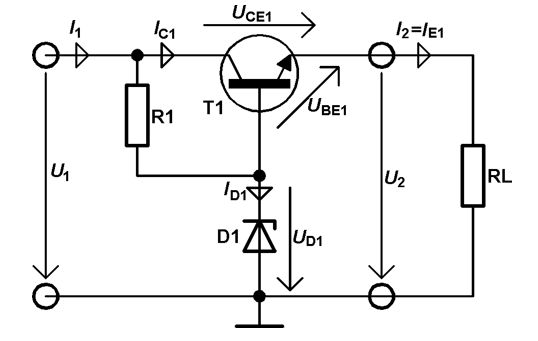
\includegraphics[width=0.55\textwidth]{img_02_param_s_tranzistorem.png}
  \caption{Parametrický stabilizátor so ZD a pomocným tranzistorom (Prednáška 2, Slide 18)}
  \label{fig:param_tranzistor}
\end{figure}

%%%%%%%%%%%%%%%%%%%%%%%%%%%%%%%%%%%%%%%%%%%%%%%%%%%
\chapter{Spojité lineárne stabilizátory}
%%%%%%%%%%%%%%%%%%%%%%%%%%%%%%%%%%%%%%%%%%%%%%%%%%%

\textit{Okruh: Spojité lineární stabilizátory, zapojení, stabilita, vlastnosti integrovaných verzí.}

\section{Princíp -- spätnoväzbová regulácia}

Lineárny (zpětnovazební) stabilizátor je v podstate \textbf{riadený odpor v sérii so záťažou}. Tento ``odpor'' je výkonový tranzistor, ktorý riadi zosilňovač odchýlky -- ten porovnáva výstupné napätie s referenciou a nastavuje tranzistor tak, aby bol rozdiel čo najmenší. Tranzistor pracuje v \textbf{aktívnej oblasti} (nie v spínacom režime) -- odtiaľ názov ``spojitý'' regulátor.

\begin{figure}[H]
  \centering
  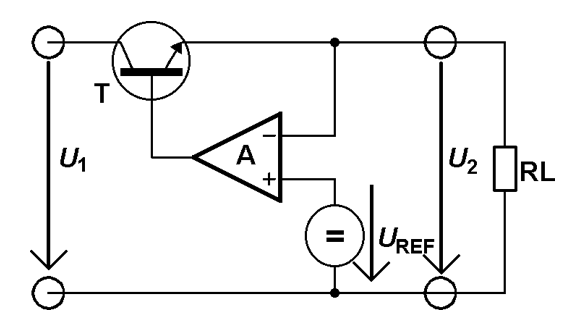
\includegraphics[width=0.65\textwidth]{img_02_LDO_blokove.png}
  \caption{Bloková schéma lineárneho stabilizátora so sériovou reguláciou (Prednáška 2, Slide 21)}
  \label{fig:ldo_blok}
\end{figure}

\section{Zapojenia}

\begin{figure}[H]
  \centering
  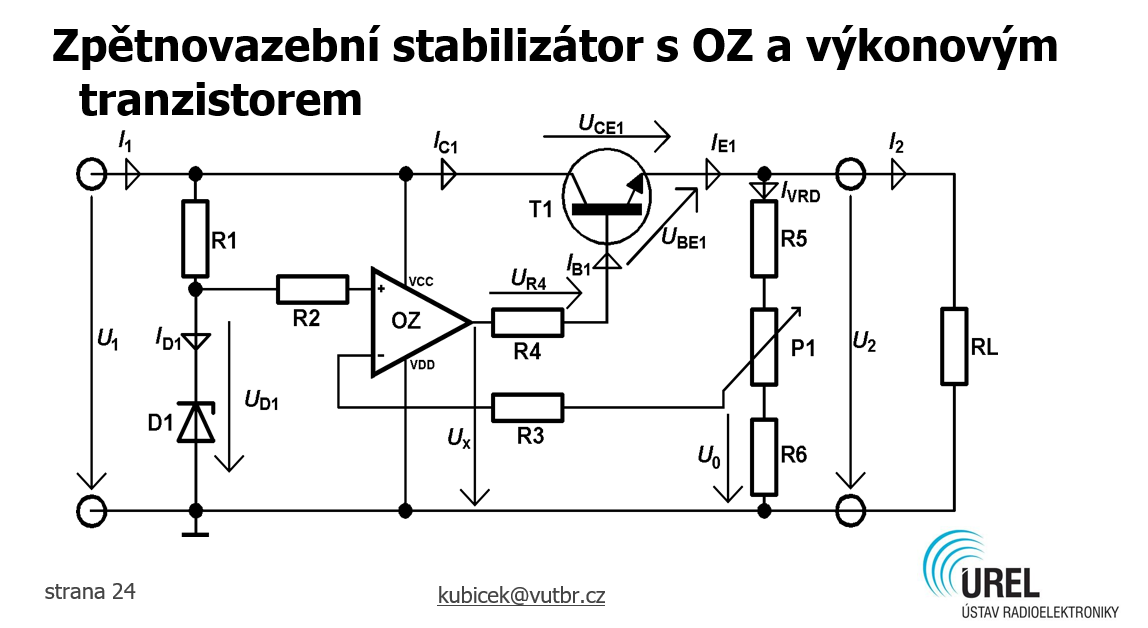
\includegraphics[width=0.65\textwidth]{img_02_stabilizator_OZ.png}
  \caption{Lineárny stabilizátor s operačným zosilňovačom a výkonovým NPN tranzistorom (Prednáška 2, Slide 24)}
  \label{fig:stab_oz}
\end{figure}

Výstupné napätie sa nastavuje odporovým deličom. OZ má veľké zosilnenie, takže aj malá odchýlka výstupného napätia od žiadanej hodnoty okamžite koriguje tranzistor.

Predchádzajúcemu zapojeniu s OZ predchádza jednoduchšia verzia -- \textbf{stabilizátor s tranzistorovým zosilňovačom odchýlky}, kde OZ nahradzuje dvojica tranzistorov. Menšie zosilnenie, ale plne diskrétne riešenie:

\begin{figure}[H]
  \centering
  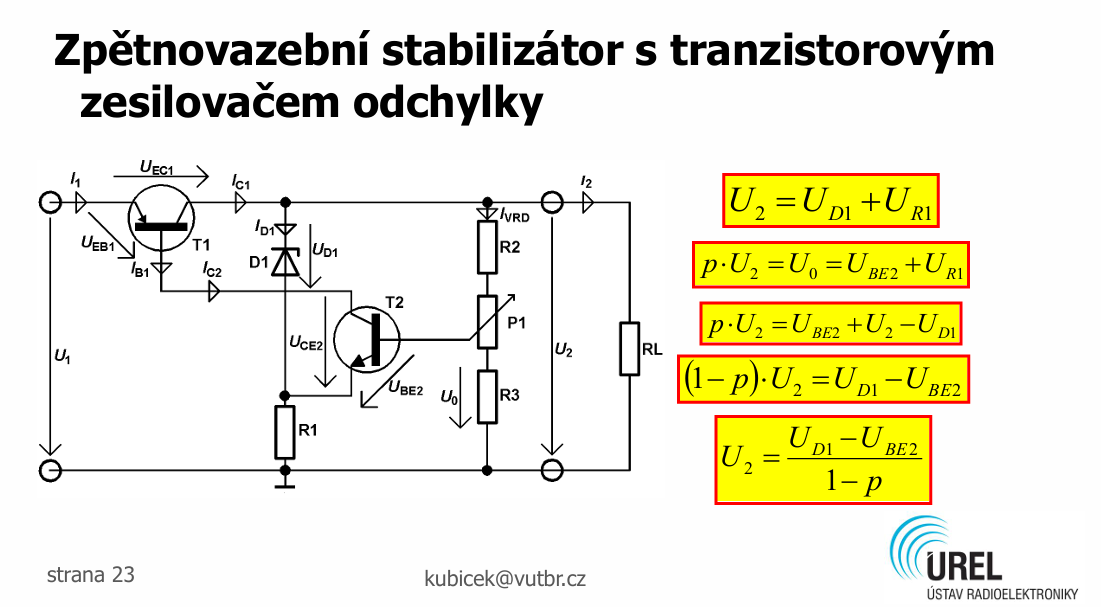
\includegraphics[width=0.65\textwidth]{img_02_stabilizator_tranzistor.png}
  \caption{Zpětnovazební stabilizátor s tranzistorovým zosilňovačom odchýlky -- diskrétna verzia (Prednáška 2, Slide 23)}
  \label{fig:stab_tranzistor}
\end{figure}

\textbf{Dropout napätie:} minimálny rozdiel $U_1 - U_2$, pri ktorom ešte stabilizátor správne pracuje. Pre NPN tranzistor je $U_{dropout} \approx U_{CE,sat} \approx 1{,}5$--$2$~V. Pre PMOS (LDO) môže byť $< 200$~mV.

\section{Integrované verzie}

\begin{itemize}
    \item \textbf{78xx / 79xx} -- pevné výstupné napätie (+5, +12, $-$5, $-$12~V...), výstupný prúd až 1~A, dropout $\approx 2$~V. Najpopulárnejšie lineárne stabilizátory vôbec.
    \item \textbf{LM317 / LM337} -- nastaviteľné napätie 1,25--37~V pomocou dvoch vonkajších odporov, až 1,5~A.
    \item \textbf{LDO (Low Dropout)} -- PMOS alebo PNP akčný člen umožňuje pracovať s minimálnym úbytkom $< 200$~mV. Príklady: LP2985, TPS7A. Ideálne pre batériové zariadenia kde je rozdiel napätí malý.
\end{itemize}

\begin{figure}[H]
  \centering
  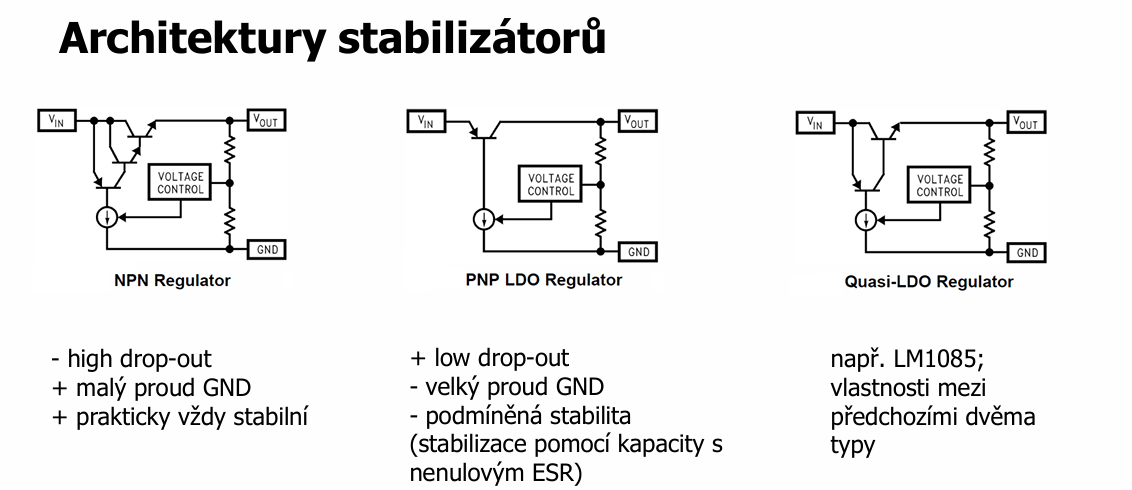
\includegraphics[width=0.75\textwidth]{img_02_ldo_architektury.png}
  \caption{Porovnanie architektúr lineárnych stabilizátorov -- NPN (veľký dropout), PNP, PMOS (LDO, malý dropout). Typ akčného člena určuje minimálny úbytok napätia (Prednáška 2, Slide 68)}
  \label{fig:ldo_arch}
\end{figure}

\textbf{Nevýhoda lineárnych stabilizátorov:} prebytočná energia ($(U_1 - U_2) \cdot I_2$) sa premení na teplo v regulačnom tranzistore. Účinnosť $\eta \approx U_2 / U_1$ -- pri veľkom rozdiele napätí je nízka.




\textbf{Výhody:} jednoduchosť, \textbf{nulové EMI rušenie} (nespínajú), veľmi rýchla odozva na zmeny záťaže, nízky šum na výstupe.

\section{Dynamické parametre a stabilita}

Keďže stabilizátor je spätnoväzbový systém, môže oscilovať pri nevhodnom návrhu. Kľúčový vplyv má \textbf{výstupný kondenzátor} -- jeho kapacita a ESR ovplyvňujú fázovú rezervu (phase margin). LDO stabilizátory s PMOS tranzistorom sú na to obzvlášť citlivé -- výrobca v katalógu vždy špecifikuje odporúčaný typ a hodnotu výstupného kondenzátora. Fázová rezerva by mala byť $\geq 45°$.

\textbf{Ďalšie dynamické parametre integrovaných stabilizátorov:}
\begin{itemize}
    \item \textbf{Line Transient Response} -- odozva na skokovu zmenu vstupného napätia; pri dobrom návrhu spôsobí len malú zmenu výstupného napätia.
    \item \textbf{Load Transient Response} -- odozva na skokovu zmenu záťaže; rýchla veľká zmena prúdu môže spôsobiť podpätie alebo prepätie. Rieši sa väčšou výstupnou kapacitou.
    \item \textbf{PSRR (Power Supply Rejection Ratio)} -- miera potlačenia zvlnenia zo vstupu na výstup; závisí od frekvencie a od rezervy nad $U_{DROP,min}$.
    \item \textbf{Kľudový odber} ($I_Q$) -- prúd odoberaný stabilizátorom pri nulovej záťaži; kritický pri batériovom napájaní.
\end{itemize}

%%%%%%%%%%%%%%%%%%%%%%%%%%%%%%%%%%%%%%%%%%%%%%%%%%%
\chapter{Spínané meniče s galvanickou väzbou}
%%%%%%%%%%%%%%%%%%%%%%%%%%%%%%%%%%%%%%%%%%%%%%%%%%%

\textit{Okruh: Spínané měniče s galvanickou vazbou, princip, zapojení silových obvodů, nábojové pumpy.}

\section{Prečo spínané meniče?}

Lineárny stabilizátor premení prebytočnú energiu na teplo -- účinnosť $\eta \approx U_2/U_1$. Spínaný menič funguje inak: \textbf{rýchlo spína tranzistor} a energiu prenáša v diskrétnych časových intervaloch cez tlumivku a kondenzátor. Vďaka tomu:
\begin{itemize}[noitemsep]
    \item Účinnosť 85--98\,\% (oproti 30--60\,\% u lineárnych stabilizátorov).
    \item Možnosť \textbf{zvyšovať} aj \textbf{invertovať} napätie, nielen znižovať.
    \item Nevýhoda: generuje elektromagnetické rušenie (EMI).
\end{itemize}

Základná štruktúra silového obvodu: \textbf{spínač (T) -- dióda (D) -- tlumivka (L)} -- kondenzátor (C). Výstupné napätie sa reguluje zmenou striedy $s = t_{ON}/T$.

\section{Znižujúci menič (Buck / Step-Down)}

Výstupné napätie je vždy \textbf{menšie} ako vstupné: $U_2 = s \cdot U_1$.

Princíp: počas $t_{ON}$ tečie prúd zo zdroja cez tlumivku do záťaže, tlumivka akumuluje energiu. Počas $t_{OFF}$ tlumivka dodáva energiu záťaži sama -- prúd tečie cez nulovaciu diódu. Kondenzátor vyhladzuje zvlnenie.

\begin{figure}[H]
  \centering
  \begin{subfigure}{0.48\textwidth}
    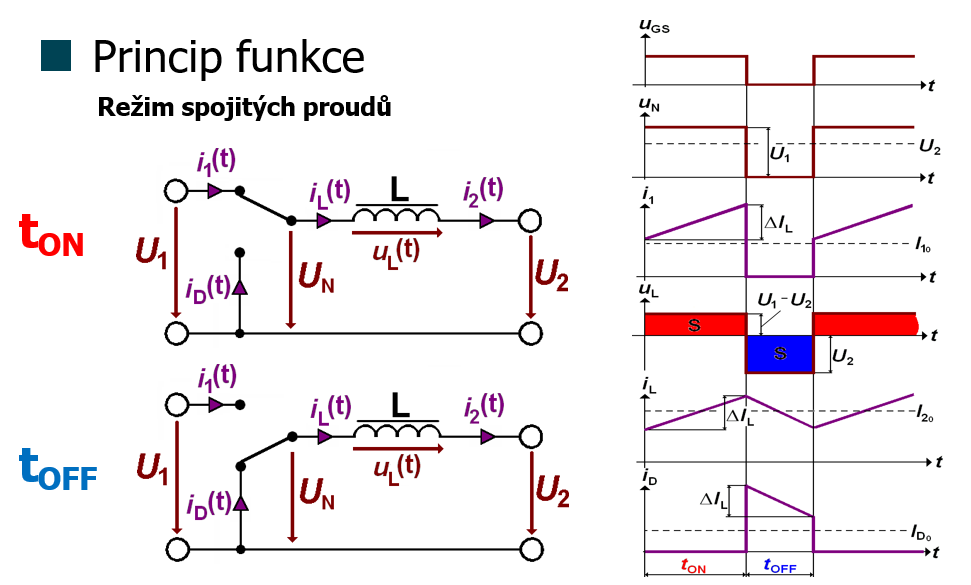
\includegraphics[width=\textwidth]{img_04_buck_priebeh.png}
    \caption{Schéma znižujúceho meniča}
  \end{subfigure}
  \hfill
  \begin{subfigure}{0.48\textwidth}
    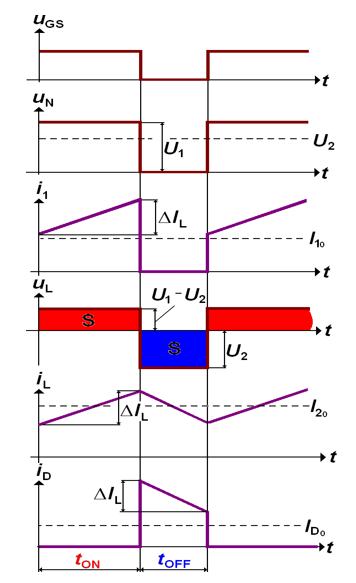
\includegraphics[width=\textwidth]{img_04_buck_priebeh2.png}
    \caption{Priebeh prúdu tlumivkou -- CCM}
  \end{subfigure}
  \caption{Znižujúci menič (Buck) -- Prednáška 4, Slide 15 a 17}
  \label{fig:buck}
\end{figure}

\textbf{CCM vs. DCM:} v režime spojitých prúdov (CCM) prúd tlumivkou neklesne na nulu. V režime nespojitých prúdov (DCM) prúd klesne na nulu pred ďalším zapnutím -- mení sa prevodový vzorec a obvod pracuje inak; nutná zmena regulácie.

\section{Spätná väzba DC/DC meniča}

Výstupné napätie sa udržuje konštantné pomocou spätnoväzbovej regulácie -- výstupné napätie sa porovnáva s referenciou a odchýlka riadi šírku impulzov (PWM regulácia striedy $s$).

\textbf{Dva základné typy spätnej väzby:}
\begin{itemize}
    \item \textbf{Napäťová spätná väzba} -- chybové napätie riadi striedu (dobu zapnutia spínača). Jednoduchší návrh, menší výstupný odpor.
    \item \textbf{Prúdová spätná väzba} -- chybové napätie riadi špičkový prúd spínačom. Rýchlejšia odozva, z princípu obmedzuje prúd v každom cykle (ochrana spínača), lepšie potlačenie Flux Walking.
\end{itemize}

\textbf{Galvanická izolácia spätnej väzby:} pri izolovaných meniačoch (Flyback, Forward) musí spätná väzba preniesť informáciu cez izoláciu. Používa sa \textbf{optočlen} (optocoupler) alebo malý \textbf{pomocný transformátor}. Optočlen typicky v kombinácii s TL431 (nastaviteľná referencia) na sekundárnej strane.

\begin{figure}[H]
  \centering
  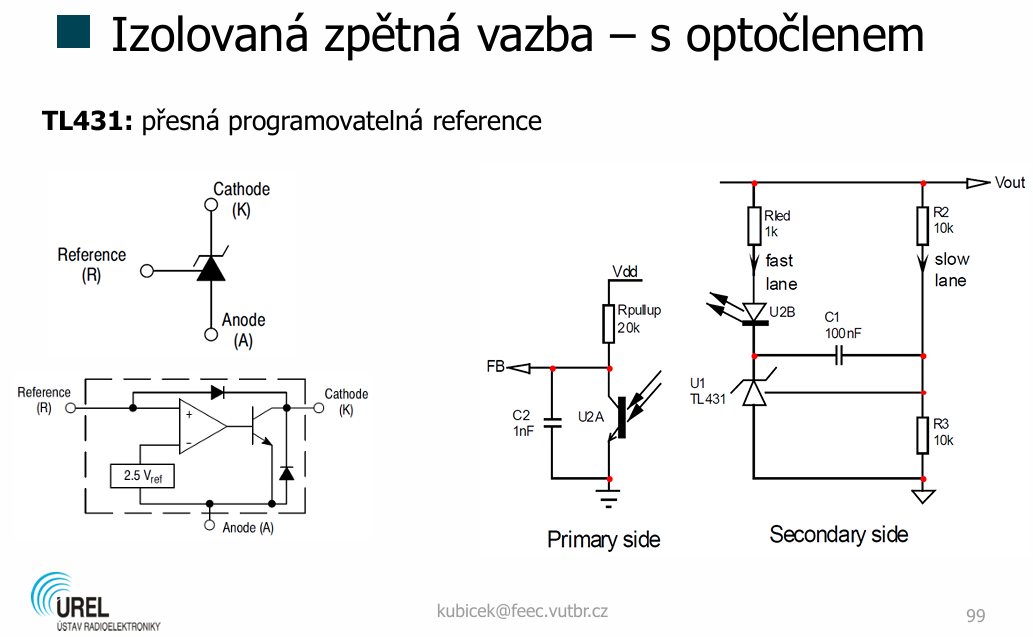
\includegraphics[width=0.70\textwidth]{img_08_zpetna_vazba_optoclen.png}
  \caption{Izolovaná spätná väzba s optočlenom a TL431 -- štandardné riešenie pre Flyback meniče (Prednáška 8, Slide 99)}



  \label{fig:zpetna_vazba}
\end{figure}

\section{Synchrónne usmerňovanie}

V základnom zapojení Buck meniča tvorí straty nulovacia dióda (úbytok $\approx 0{,}7$~V). Pri nízkych výstupných napätiach (napr. 1~V pre CPU) môžu tieto straty tvoriť desiatky percent celkového výkonu.

\textbf{Riešenie -- synchrónny menič:} nulovaciu diódu nahradíme druhým MOSFET tranzistorom, spínaným protifázne voči hlavnému tranzistoru. MOSFET má oveľa menší úbytok ($R_{DS,on} \cdot I$, typicky $<50$~mV). Výsledok: výrazne vyššia účinnosť, najmä pri nízkych výstupných napätiach a veľkých prúdoch.

Synchrónne usmerňovanie sa dnes používa štandardne vo väčšine integrovaných DC/DC meniačov.

\begin{figure}[H]
  \centering
  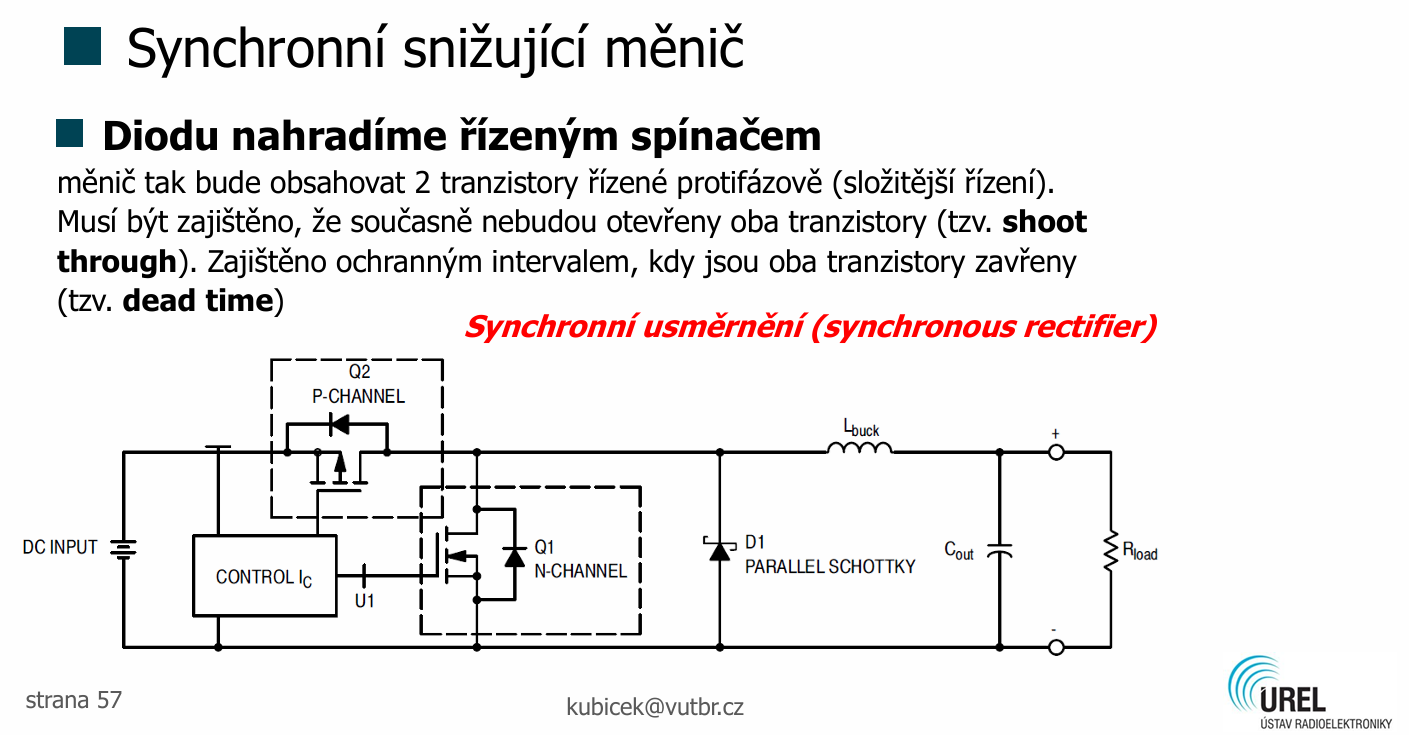
\includegraphics[width=0.65\textwidth]{img_04_sync_buck.png}
  \caption{Synchrónny znižujúci menič -- nulovacia dióda nahradená druhým MOSFET tranzistorom (Prednáška 4, Slide 57)}
  \label{fig:sync_buck}
\end{figure}

\section{Zvyšujúci menič (Boost / Step-Up)}

Výstupné napätie je vždy \textbf{väčšie} ako vstupné: $U_2 = U_1 / (1-s)$.

Počas $t_{ON}$ sa energia akumuluje v tlumivke (spínač skratuje tlumivku na GND). Počas $t_{OFF}$ tlumivka uvoľní energiu -- napätie na jej svorkách sa sčíta s vstupným napätím a nabije výstupný kondenzátor na vyššiu hodnotu. Typické použitie: batériové zariadenia (napr. 3~V $\to$ 5~V).

\begin{figure}[H]
  \centering
  \begin{subfigure}{0.48\textwidth}
    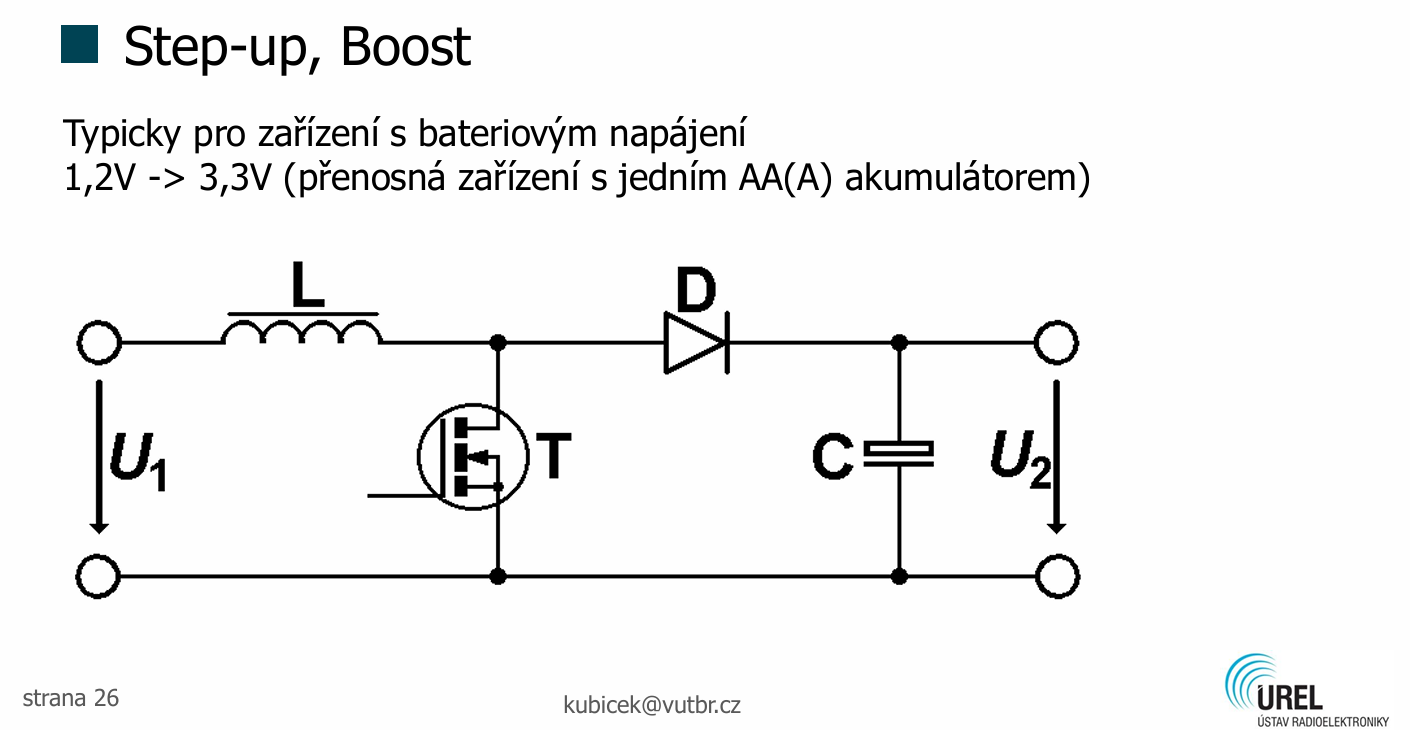
\includegraphics[width=\textwidth]{img_04_boost_schema.png}
    \caption{Schéma zvyšujúceho meniča}
  \end{subfigure}
  \hfill
  \begin{subfigure}{0.48\textwidth}
    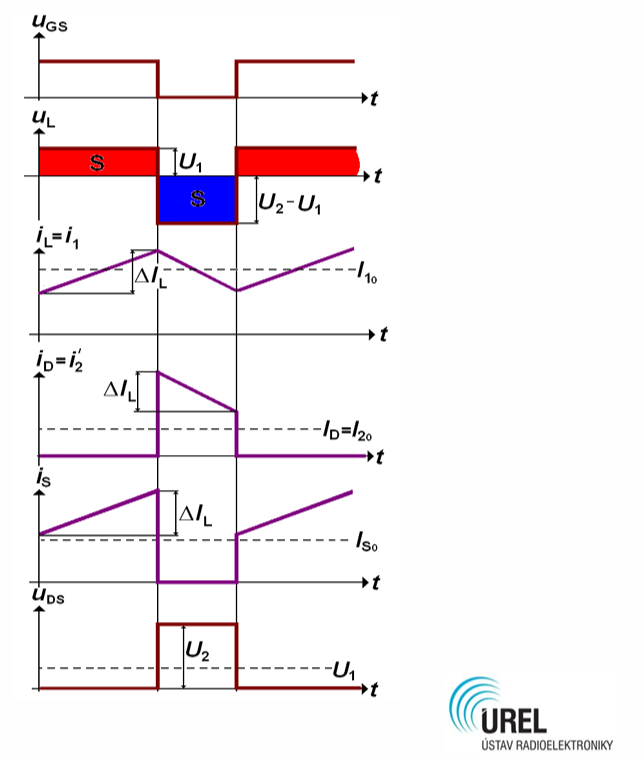
\includegraphics[width=\textwidth]{img_04_boost_priebeh.png}
    \caption{Priebeh prúdu tlumivkou}
  \end{subfigure}
  \caption{Zvyšujúci menič (Boost) -- Prednáška 4, Slide 26 a 28}
  \label{fig:boost}
\end{figure}

\section{Invertujúci menič (Buck-Boost)}

Výstupné napätie je \textbf{opačnej polarity} ako vstupné: $U_2 = -s/(1-s) \cdot U_1$.

Výstupné napätie modulom môže byť menšie aj väčšie ako vstup. Využíva sa pre získanie záporného napájania z kladného zdroja.

\begin{figure}[H]
  \centering
  \begin{subfigure}{0.48\textwidth}
    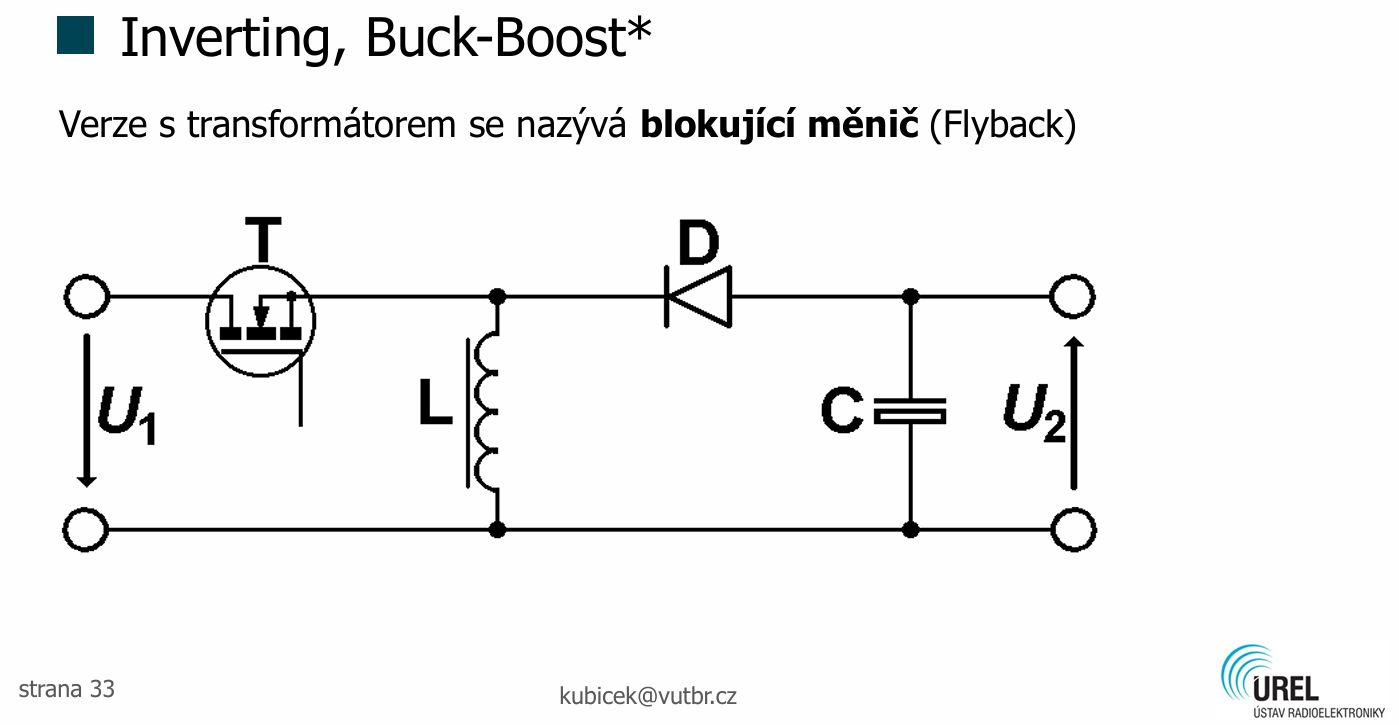
\includegraphics[width=\textwidth]{img_04_buckboost_schema.png}
    \caption{Schéma invertujúceho meniča}
  \end{subfigure}
  \hfill
  \begin{subfigure}{0.48\textwidth}
    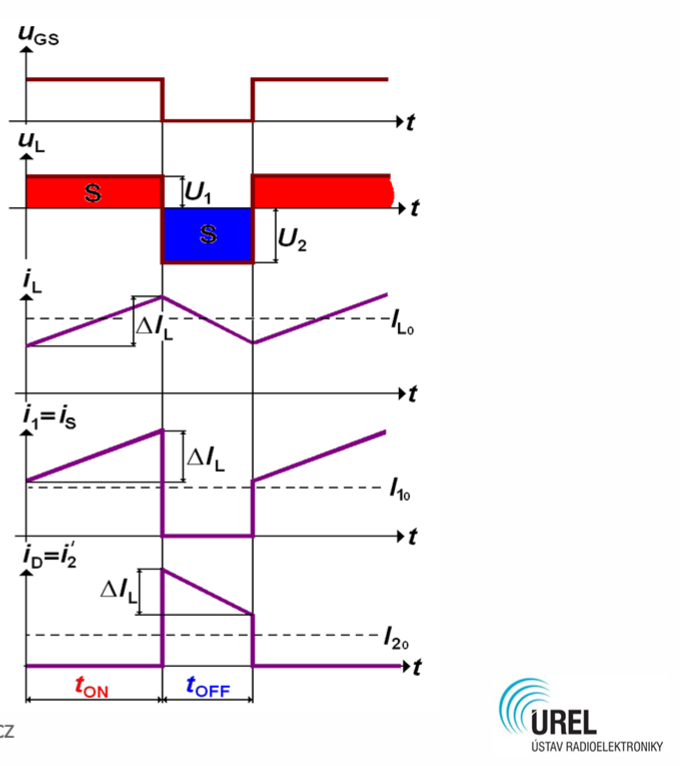
\includegraphics[width=\textwidth]{img_04_buckboost_priebeh.png}
    \caption{Priebeh prúdov}
  \end{subfigure}
  \caption{Invertujúci menič (Buck-Boost) -- Prednáška 4, Slide 33 a 35}
  \label{fig:buckboost}
\end{figure}

\begin{figure}[H]
  \centering
  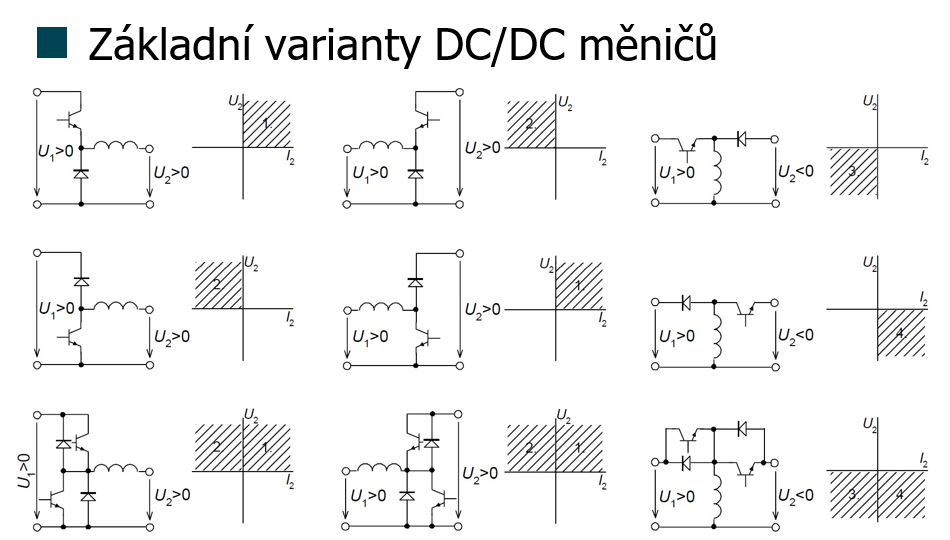
\includegraphics[width=0.75\textwidth]{img_04_dc_dc_typy.png}
  \caption{Porovnanie základných neizolovaných DC/DC meniačov -- Buck, Boost, Buck-Boost (Prednáška 4, Slide 12)}
  \label{fig:dcdc_typy}
\end{figure}

\section{Nábojové pumpy}

Špeciálny prípad neizolovaného meniča -- \textbf{bez tlumivky}, len kondenzátory a spínače. Vhodný iba pre malé výkony (jednotky až desiatky mA).

Princíp zdvojovača:
\begin{enumerate}[noitemsep]
    \item \textbf{Fáza nabíjania:} kondenzátor $C_1$ sa nabije na vstupné napätie $U_1$.
    \item \textbf{Fáza prenosu:} $C_1$ sa prepne do série so vstupom $\to$ výstup dosiahne $U_2 \approx 2 \cdot U_1$.
\end{enumerate}

\begin{figure}[H]
  \centering
  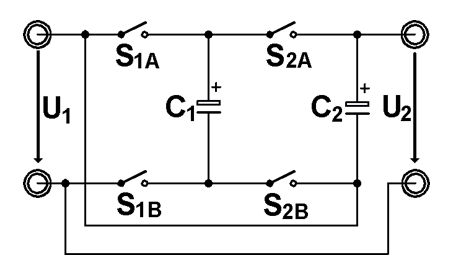
\includegraphics[width=0.65\textwidth]{img_04_nabojova_pumpa.png}
  \caption{Nábojová pumpa -- zdvojovač napätia, dve fázy činnosti (Prednáška 4, Slide 66)}
  \label{fig:nabojova_pumpa}
\end{figure}

Integrované obvody umožňujú aj inverziu ($U_2 = -U_1$) alebo násobok $1{,}5\times$. Príklady: MAX660, ICL7660.

%%%%%%%%%%%%%%%%%%%%%%%%%%%%%%%%%%%%%%%%%%%%%%%%%%%
\chapter{Spínané meniče s transformátorom}
%%%%%%%%%%%%%%%%%%%%%%%%%%%%%%%%%%%%%%%%%%%%%%%%%%%

\textit{Okruh: Spínané měniče s transformátorem, princip, zapojení silových obvodů, vlastnosti.}

\section{Prečo transformátor?}

Transformátor v spínanom zdroji poskytuje:
\begin{itemize}[noitemsep]
    \item \textbf{Galvanická izolácia} -- výstup je bezpečne oddelený od vstupu (povinné pre zariadenia napájané zo siete 230~V).
    \item \textbf{Ľubovolný prevod napätia} -- veľké prevody (napr. 230~V $\to$ 3,3~V) jednoducho pomerom závitov.
    \item \textbf{Viacnásobné výstupy} -- viac sekundárnych vinutí, každé na iné napätie.
\end{itemize}

\section{Blokujúci menič (Flyback)}

Najpopulárnejšia izolovaná topológia pre výkony do $\approx 200$~W. Vychádza z invertujúceho meniča -- transformátor tu nefunguje ako klasický transformátor, ale ako \textbf{tlumivka s dvoma vinutiami (cívka v proudovém módu)}:

\begin{itemize}
    \item Počas \textbf{zapnutia} tranzistora tečie prúd primárnym vinutím a \textbf{akumuluje energiu v jadre}. Sekundárna dióda je v závernom smere -- do záťaže nič netečie.
    \item Počas \textbf{vypnutia} sa polarita na transformátore otočí, sekundárna dióda sa otvorí a \textbf{energia sa prenesie z jadra do záťaže}.
\end{itemize}

Keďže jadro musí akumulovať energiu ako tlumivka, \textbf{vyžaduje vzduchov. medzeru} (inak by sa nasýtilo).

\begin{figure}[H]
  \centering
  \begin{subfigure}{0.48\textwidth}
    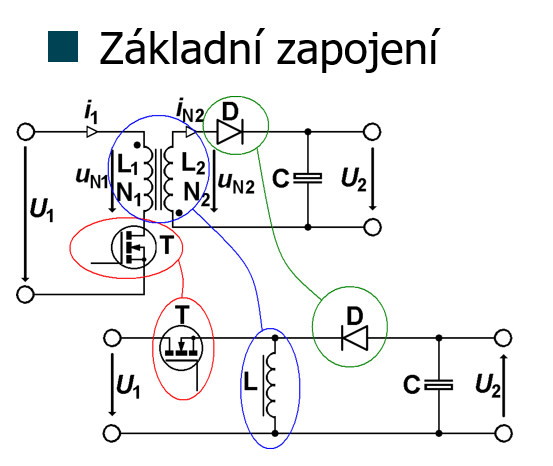
\includegraphics[width=\textwidth]{img_05_flyback_schema.png}
    \caption{Schéma Flyback meniča}
  \end{subfigure}
  \hfill
  \begin{subfigure}{0.48\textwidth}
    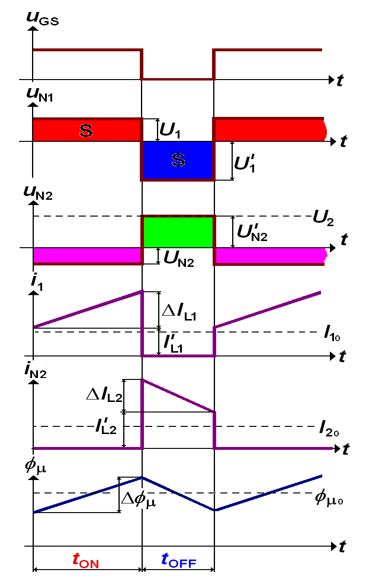
\includegraphics[width=\textwidth]{img_05_flyback_priebeh.png}
    \caption{Priebeh prúdov a napätí}
  \end{subfigure}
  \caption{Blokujúci menič (Flyback) -- Prednáška 5, Slide 4 a 5}
  \label{fig:flyback}
\end{figure}

\textbf{Výhody:} jednoduchosť (minimum súčiastok), ľahké viacnásobné výstupy, galvanická izolácia. \textbf{Nevýhody:} horšie využitie jadra (vzduchová medzera), väčší transformátor, väčšie EMI.

\section{Propustný menič (Forward)}

Vychádza zo znižujúceho meniča (Buck). Energia sa prenáša \textbf{priamo počas zapnutia} tranzistora -- odtiaľ ``propustný''. Na sekundári je rovnaká štruktúra ako u Buck meniča (dióda D0 + tlumivka L + kondenzátor C). Prevodový vzťah: $U_2 = U_1 \cdot (N_2/N_1) \cdot s$.

Transformátor pracuje ako skutočný transformátor -- \textbf{bez vzduchov. medzery}. Po vypnutí tranzistora je transformátor namagnetizovaný a musí sa demagnetizovať -- bez toho by sa jadro cyklus od cyklu nasycovalo. Riešenia demagnetizácie:
\begin{itemize}[noitemsep]
    \item \textbf{Tretie (reset) vinutie $N_3$} -- energia sa cez diódu $D_1$ vráti do zdroja. Podmienka: $t_{DEM} \leq t_{OFF}$, čiže max. strida $s \leq N_1/N_3 / (1 + N_1/N_3)$.
    \item \textbf{Zenerova dióda} -- energia rozptylovej indukčnosti sa disipuje (straty).
    \item \textbf{Two-switch Forward} -- dva tranzistory, energia sa vracia cez diódy do zdroja, $U_{DS,max} = U_1$.
    \item \textbf{Active Clamp Forward} -- aktívny spínač s kondenzátorom, umožňuje ZVS spínanie.
\end{itemize}

Obrázok nižšie ukazuje variant s \textbf{reset vinutím $N_3$}: primárne vinutie $N_1$ je budené tranzistorom T. Počas $t_{ON}$ tečie energia cez $N_1 \to N_2$ priamo do záťaže. Počas $t_{OFF}$ sa polarita otočí, dióda $D_1$ sa otvorí a demagnetizačný prúd tečie späť do zdroja cez vinutie $N_3$.

\begin{figure}[H]
  \centering
  \begin{subfigure}{0.48\textwidth}
    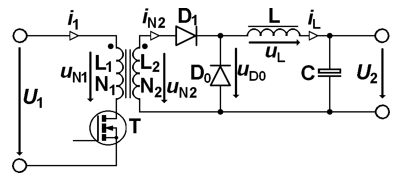
\includegraphics[width=\textwidth]{img_05_forward_demagnetizace.png}
    \caption{Schéma: primár $N_1$ (T), reset vinutie $N_3$ (D1), sekundár $N_2$ (D0, L, C)}
  \end{subfigure}
  \hfill
  \begin{subfigure}{0.48\textwidth}
    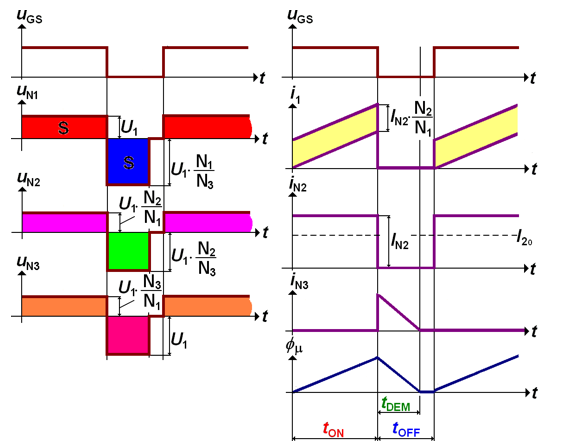
\includegraphics[width=\textwidth]{img_05_forward_demagnetizace_priebeh.png}
    \caption{Priebeh: fáza $t_{ON}$ (prenos energie) a $t_{DEM}$ (demagnetizácia cez $N_3$)}
  \end{subfigure}
  \caption{Propustný menič (Forward) s reset vinutím $N_3$ -- Prednáška 5, Slide 22 a 23}
  \label{fig:forward}
\end{figure}

\subsection{Two-switch Forward}

Variant s dvoma tranzistormi (T1 hore, T2 dole) eliminuje vysoké napäťové namáhanie -- každý tranzistor je namáhaný len $U_1$ (nie $2U_1$ ako pri jednočinnom Forward). Energia rozptylovej indukčnosti sa vracia do zdroja cez diódy, takže nenámaháha ani tranzistory ani snubbery:

\begin{figure}[H]
  \centering
  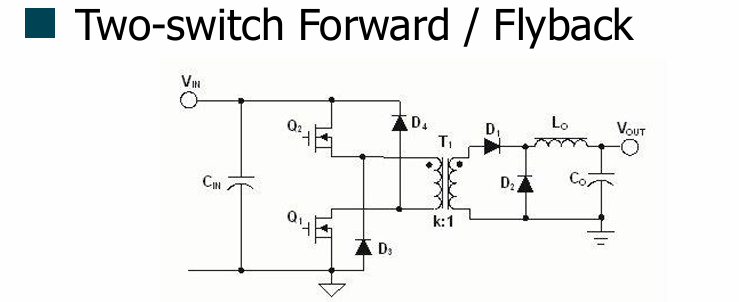
\includegraphics[width=0.65\textwidth]{img_05_two_switch_forward.png}
  \caption{Two-switch Forward -- T1 a T2 spínajú súčasne, demagnetizácia prebieha cez diódy späť do zdroja, $U_{DS,max} = U_1$ (Prednáška 5, Slide 27)}
  \label{fig:two_switch_forward}
\end{figure}



%%%%%%%%%%%%%%%%%%%%%%%%%%%%%%%%%%%%%%%%%%%%%%%%%%%
\chapter{Mostíkové meniče}
%%%%%%%%%%%%%%%%%%%%%%%%%%%%%%%%%%%%%%%%%%%%%%%%%%%

\textit{Okruh: Můstkové měniče, princip, zapojení silových obvodů, vlastnosti.}

\section{Prečo mostíkové topológie?}

Flyback a Forward meniče magnetizujú jadro len \textbf{jedným smerom} -- využíva sa len polovica hysteréznej slučky jadra. Mostíkové meniče magnetizujú jadro \textbf{oboma smermi} striedavo -- dvojnásobné využitie jadra, transformátor môže byť menší. Preto sa mostíkové meniče používajú pre vyššie výkony (stovky W až desiatky kW).

\section{Push-Pull menič}

Dva tranzistory pracujúce na jednom transformátore striedavo. Každý tranzistor magnetizuje jadro v opačnom smere. Výsledok: výstupné pulzy majú dvojnásobnú frekvenciu, jadro je využité symetricky. Každý tranzistor je namáhaný napätím $2 U_1$.

\textbf{Problém Flux Walking:} ak striedy oboch tranzistorov nie sú dokonale rovnaké, akumuluje sa jednosmerná zložka magnetizácie a jadro sa postupne nasýti. Riešenie: prúdová regulácia (prúdový mód), blokovací kondenzátor.

\begin{figure}[H]
  \centering
  \begin{subfigure}{0.48\textwidth}
    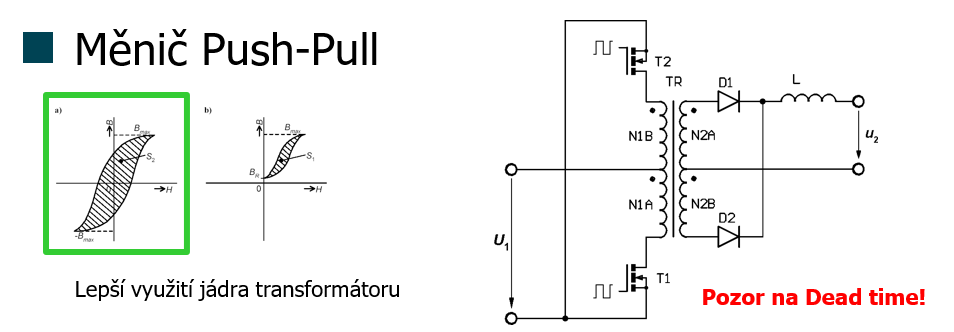
\includegraphics[width=\textwidth]{img_05_push_pull.png}
    \caption{Schéma Push-Pull meniča}
  \end{subfigure}
  \hfill
  \begin{subfigure}{0.48\textwidth}
    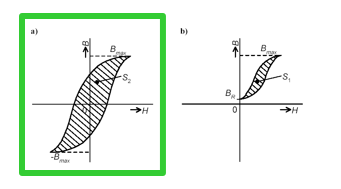
\includegraphics[width=\textwidth]{img_05_push_pull_priebeh.png}
    \caption{Priebeh prúdov a magnetizácie}
  \end{subfigure}
  \caption{Push-Pull menič -- Prednáška 5, Slide 35}
  \label{fig:push_pull}
\end{figure}

\section{Polmostíkový menič (Half-Bridge)}

Dva tranzistory (horný a dolný) sa striedajú. Na primárnom vinutí sa striedavo objavuje $+U_1/2$ a $-U_1/2$. \textbf{Blokovací kondenzátor} v sérii s primárom \textbf{automaticky zabraňuje Flux Walking} -- prirodzene odfiltruje jednosmernú zložku. Tranzistory sú namáhané len $U_1$ (oproti $2 U_1$ u Push-Pull).

\textbf{Dead time} (mŕtvy čas) medzi spínaním horného a dolného tranzistora je nevyhnutný -- zabraňuje priamemu skratu napájacieho napätia (tzv. shoot-through).

\begin{figure}[H]
  \centering
  \begin{subfigure}{0.48\textwidth}
    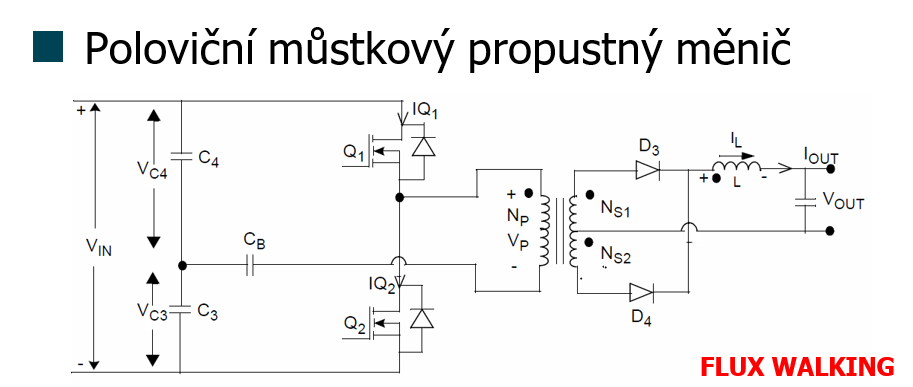
\includegraphics[width=\textwidth]{img_05_half_bridge.png}
    \caption{Schéma Half-Bridge meniča}
  \end{subfigure}
  \hfill
  \begin{subfigure}{0.48\textwidth}
    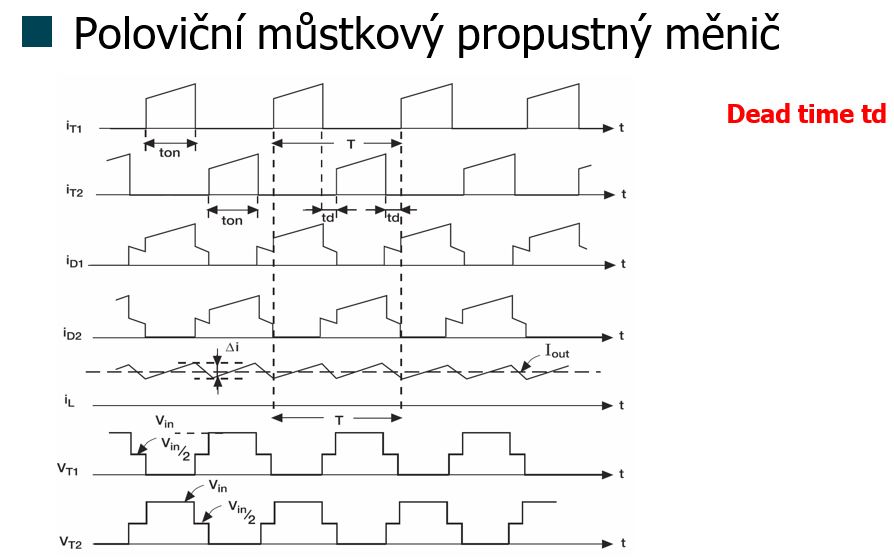
\includegraphics[width=\textwidth]{img_05_half_bridge_priebeh.png}
    \caption{Priebeh -- Dead time}
  \end{subfigure}
  \caption{Polmostíkový menič Half-Bridge -- Prednáška 5, Slide 36 a 41}
  \label{fig:halfbridge}
\end{figure}

\section{Plný mostík (Full-Bridge)}

Štyri tranzistory v H-mostíkovom zapojení -- dve diagonály sa striedavo spínajú. Na primárnom vinutí sa objavuje plné $+U_1$ a $-U_1$ -- dvojnásobok oproti Half-Bridge. To umožňuje preniesť dvojnásobný výkon pri rovnakom transformátore. Tranzistory sú tiež namáhané len $U_1$.

\begin{figure}[H]
  \centering
  \begin{subfigure}{0.48\textwidth}
    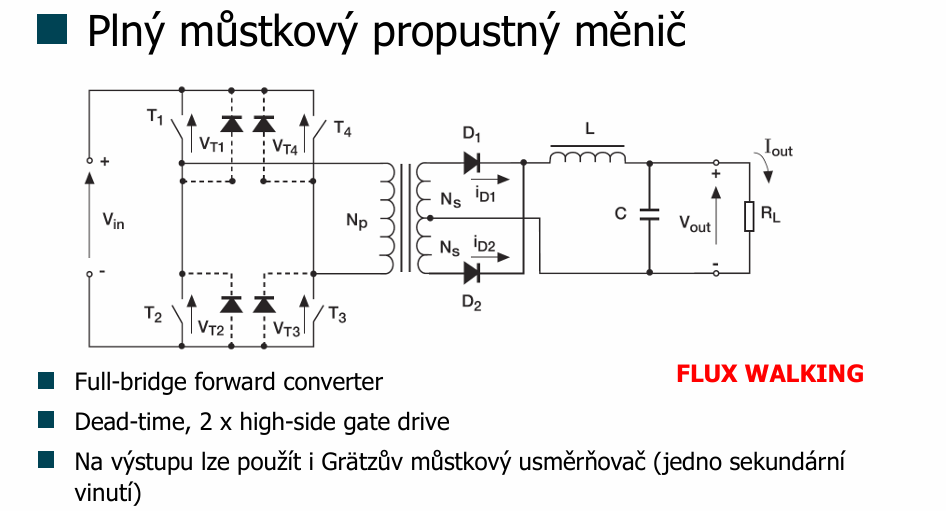
\includegraphics[width=\textwidth]{img_05_full_bridge.png}
    \caption{Schéma Full-Bridge meniča}
  \end{subfigure}
  \hfill
  \begin{subfigure}{0.48\textwidth}
    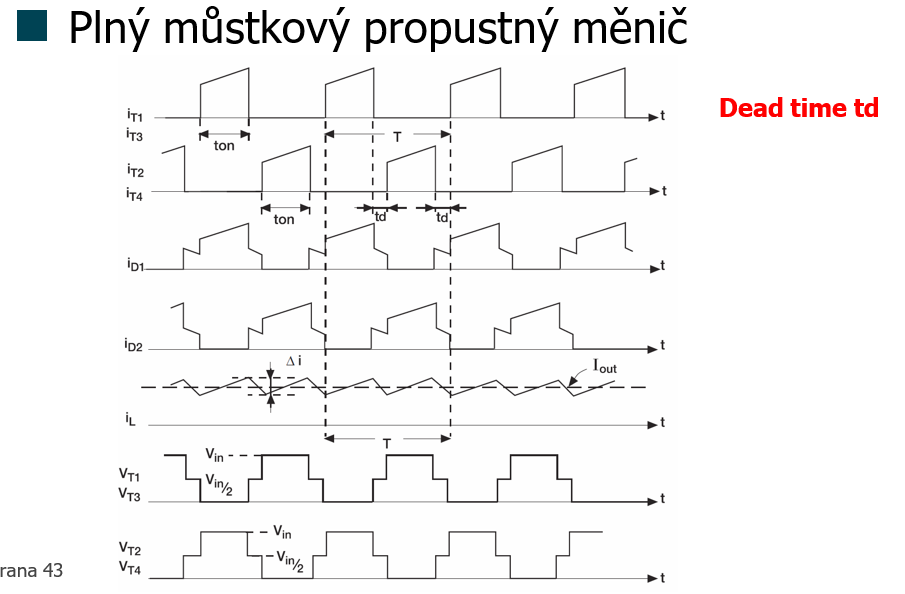
\includegraphics[width=\textwidth]{img_05_full_bridge_priebeh.png}
    \caption{Priebeh napätia na primárnom vinutí}
  \end{subfigure}
  \caption{Plný mostík Full-Bridge -- Prednáška 5, Slide 42 a 43}
  \label{fig:fullbridge}
\end{figure}

\begin{center}
\begin{tabular}{llll}
\toprule
\textbf{Topológia} & \textbf{Počet T} & \textbf{Max. $U_{DS}$} & \textbf{Typický výkon} \\
\midrule
Push-Pull    & 2 & $2 U_1$ & 100--500~W \\
Half-Bridge  & 2 & $U_1$   & 200~W -- 1~kW \\
Full-Bridge  & 4 & $U_1$   & 500~W -- desiatky kW \\
\bottomrule
\end{tabular}
\end{center}

%%%%%%%%%%%%%%%%%%%%%%%%%%%%%%%%%%%%%%%%%%%%%%%%%%%
\chapter{Elektrochemické zdroje, chladenie, jistenie, PFC}
%%%%%%%%%%%%%%%%%%%%%%%%%%%%%%%%%%%%%%%%%%%%%%%%%%%

\textit{Okruh: Elektrochemické zdroje proudu, chlazení součástek, přepěťové a nadproudové jištění napájecích zdrojů, korektory účiníku.}

\section{Elektrochemické zdroje prúdu}

\textbf{Primárne články} (nenabíjateľné):

\begin{center}
\begin{tabular}{lll}
\toprule
\textbf{Typ} & \textbf{Napätie/článok} & \textbf{Poznámka} \\
\midrule
Zinko-uhlíkový (Leclanché) & 1,5~V & Lacný, malá kapacita, horšie za chladu \\
Alkalický (MnO$_2$) & 1,5~V & Bežný, dobrá kapacita, dlhá trvanlivosť \\
Lítiový (Li-MnO$_2$) & 3,0~V & Najväčšia kapacita, 10+ rokov skladovania \\
\bottomrule
\end{tabular}
\end{center}

\textbf{Sekundárne články} (nabíjateľné -- akumulátory):

\begin{center}
\begin{tabular}{lllll}
\toprule
\textbf{Typ} & \textbf{U/čl.} & \textbf{Sp. energia} & \textbf{Cykly} & \textbf{Poznámka} \\
\midrule
Pb (olověný) & 2,0~V & 30--40~Wh/kg & $>300$ & Lacný, ťažký, veľké zálohy \\
NiCd         & 1,2~V & 40--60~Wh/kg & $>500$ & Memory effect, Cd je toxický \\
NiMH         & 1,2~V & 100~Wh/kg    & $>300$ & Bežné AA/AAA \\
Li-Ion       & 3,6~V & 200~Wh/kg    & $>1200$ & Smartfóny, notebooky \\
LiFePO4      & 3,3~V & 110~Wh/kg    & $>2000$ & Bezpečný, dlhá životnosť \\
\bottomrule
\end{tabular}
\end{center}

\textbf{Nabíjanie Li-Ion:} fáza \textbf{CC} (konštantný prúd) až do 4,2~V/článok, potom fáza \textbf{CV} (konštantné napätie) kým prúd neklesne na $\approx C/10$. Nikdy neprekročiť 4,2~V a nevybíjať pod 2,5~V/článok -- inak trvalé poškodenie.

\textbf{Superkapacitory:} extrémne vysoký počet cyklov ($10^5$--$10^6$), rýchle nabitie/vybitie, ale nízka merná energia ($\approx 5$~Wh/kg). Vhodné ako krátkodobý výkonový buffer.

\section{Chladzenie súčiastok}

Každý výkonový prvok generuje teplo. Teplota priechodu $T_j$ nesmie prekročiť maximum (typicky 125--150~°C u Si). Teplo sa odvádza cez sériu tepelných odporov:

\[ T_j = T_a + P_D \cdot (R_{th,jc} + R_{th,hi} + R_{th,cl} + R_{th,ca}) \]

kde $R_{th,jc}$ je odpor priechod-puzdro, $R_{th,hi}$ odpor izolačnej podložky, $R_{th,cl}$ odpor chladiča a $R_{th,ca}$ odpor chladič-vzduch.

\begin{figure}[H]
  \centering
  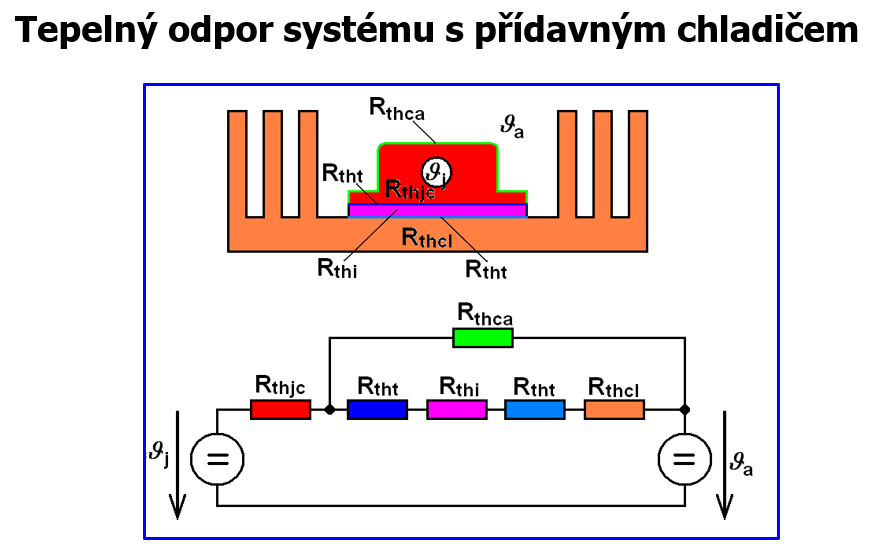
\includegraphics[width=0.65\textwidth]{img_03_chladenie_schema.png}
  \caption{Tepelný model chladiacieho systému -- náhradný obvod s tepelnými odpormi (Prednáška 3, Slide 7)}
  \label{fig:chlazeni}
\end{figure}

\textbf{Typy chladenia:}
\begin{itemize}[noitemsep]
    \item \textbf{Pasívne na DPS} -- pre straty $<1$~W.
    \item \textbf{Pasívny hliníkový chladič} -- najpoužívanejší, $R_{th} \approx 1{,}5$--$20$~K/W.
    \item \textbf{Aktívny chladič s ventilátorom} -- nižší $R_{th}$, závisí na prietoku.
    \item \textbf{Heat pipes} -- efektívny prenos tepla na diaľku.
\end{itemize}
Medzi súčiastkou a chladičom je \textbf{izolačná podložka} (slída, keramika, silikónová fólia) a tepelná pasta pre minimalizáciu kontaktného odporu.

\section{Prepäťové a nadprúdové jistenie}

\textbf{Nadprúdová ochrana:}
\begin{itemize}
    \item \textbf{Tavná poistka} -- jednoduchá, jednorazová. T (pomalá) pre záťaže s veľkým záberovým prúdom (motory), F (rýchla) pre citlivé obvody.
    \item \textbf{PTC poistka (Polyfuse/Polyswitch)} -- pri prehriatí vzrastie odpor a obmedzí prúd. Po ochladení sa automaticky obnoví. Vhodná tam, kde výmena nie je možná.
    \item \textbf{Elektronická prúdová ochrana} -- sníma prúd cez $R_{shunt}$ a pri prekročení limitu vypne výstup. Najrýchlejšia a nastaviteľná.
\end{itemize}

\textbf{Prepäťová ochrana:}
\begin{itemize}
    \item \textbf{TVS dióda (Transil)} -- správa sa ako Zenerova dióda, ale absorbuje oveľa väčšie energetické impulzy (blesk, ESD). Dostupné jednosmerné aj obojsmerné.
    \item \textbf{Crowbar (tyristorový skrat)} -- pri prepätí tyristor skratuje výstup. \textbf{Vždy musí byť v kombinácii s prúdovou poistkou} -- inak by skrat zničil zdroj.
    \item Typické poradie ochrán od vstupu: bleskojistka $\to$ TVS $\to$ Zenerova dióda.
\end{itemize}

\section{Korektor účiníka (PFC)}

\textbf{Problém:} bežný napájací zdroj (usmerňovač + filtračný kondenzátor) odoberá zo siete prúd v krátkych pulzoch namiesto sínusoidy. To spôsobuje harmonické skreslenie, deformačný jalový výkon a rušenie siete. Norma \textbf{IEC 61000-3-2} obmedzuje harmonické zložky pre zariadenia nad 75~W.

\textbf{Účiník} ($PF$) vyjadruje, aký podiel zdanlivého výkonu je skutočný aktívny výkon. Pre čistú sínusoidu $PF = 1$. Bežný zdroj bez PFC: $PF \approx 0{,}5$--$0{,}65$.

\textbf{Pasívne PFC:} LC filter pred usmerňovačom, $PF \leq 0{,}7$. Lacné, ťažké, obmedzená účinnosť.

\textbf{Aktívne PFC:} pomocný \textbf{Boost menič} pred hlavným zdrojom tvaruje vstupný prúd do tvaru sínusoidy synchronizovanej so sieťovým napätím. Výsledok: $PF > 0{,}99$. Povinné pre zariadenia nad 75~W.

\begin{figure}[H]
  \centering
  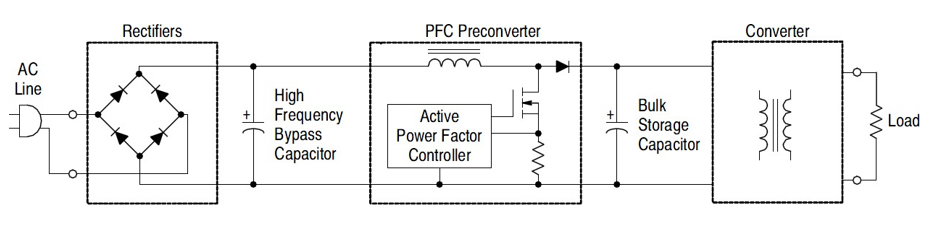
\includegraphics[width=0.70\textwidth]{img_08_aktivni_PFC.png}
  \caption{Aktívny PFC -- Boost menič pred hlavným DC/DC zdrojom tvaruje odoberaný prúd (Prednáška 8, Slide 86)}
  \label{fig:pfc}
\end{figure}

%%%%%%%%%%%%%%%%%%%%%%%%%%%%%%%%%%%%%%%%%%%%%%%%%%%
\chapter{Parametre výkonových tranzistorov a prechodové javy}
%%%%%%%%%%%%%%%%%%%%%%%%%%%%%%%%%%%%%%%%%%%%%%%%%%%

\textit{Okruh: Parametry výkonových tranzistorů z hlediska napájecích zdrojů, přechodové jevy při spínání a vypínání indukčních zátěží a jejich potlačení.}

\section{Prehľad výkonových spínačov}

\begin{center}
\begin{tabular}{lllll}
\toprule
\textbf{Prvok} & \textbf{Riadenie} & \textbf{Výkon} & \textbf{Frekvencia} & \textbf{Použitie} \\
\midrule
Tyristor (SCR) & prúdové (Gate) & veľmi veľký & do 10~kHz  & AC riadenie, usmerňovače \\
GTO / IGCT     & prúdové (vypínateľný) & veľmi veľký & do 10~kHz & veľké pohony \\
Triak          & prúdové & stredný & nízka & AC regulátory, stmievače \\
BJT            & prúdové (báza) & stredný & do stoviek~kHz & lin. stabilizátory \\
MOSFET         & napäťové (Gate) & stredný & až MHz & spínané zdroje \\
IGBT           & napäťové (Gate) & veľký & do 100~kHz & pohony, zváracie zdroje \\
\bottomrule
\end{tabular}
\end{center}

\section{MOSFET}

MOSFET je dnes \textbf{najrozšírenejší spínač} v spínaných zdrojoch. Ovláda sa napätím na Gate -- nevyžaduje trvalý budiaci prúd (len nabíjací prúd kapacity Gate pri každom spínaní). Kľúčové parametre:

\begin{itemize}
    \item \textbf{$R_{DS,on}$} -- odpor kanálu v sepnutom stave. Čím menší, tým menšie vodivostné straty. Rastie s teplotou (kladný TC) -- výhoda pri paralelnom zapojení (zabraňuje tepelnému runaway).
    \item \textbf{$U_{GS,th}$} -- prahové napätie, od ktorého sa začína otvárať. Typicky 2--4~V.
    \item \textbf{$C_{iss}$, $Q_g$} -- vstupná kapacita a celkový náboj Gate. Určujú budiaci výkon a rýchlosť spínania.
    \item \textbf{$U_{DS,max}$} -- maximálne závěrné napätie drain-source.
    \item \textbf{Parazitná body dióda} -- každý N-channel MOSFET má integrovanú antiparalelnu diódu. Výhodná pre ZVS, ale pomalšia ako externá Schottkyho dióda.
\end{itemize}

\begin{figure}[H]
  \centering
  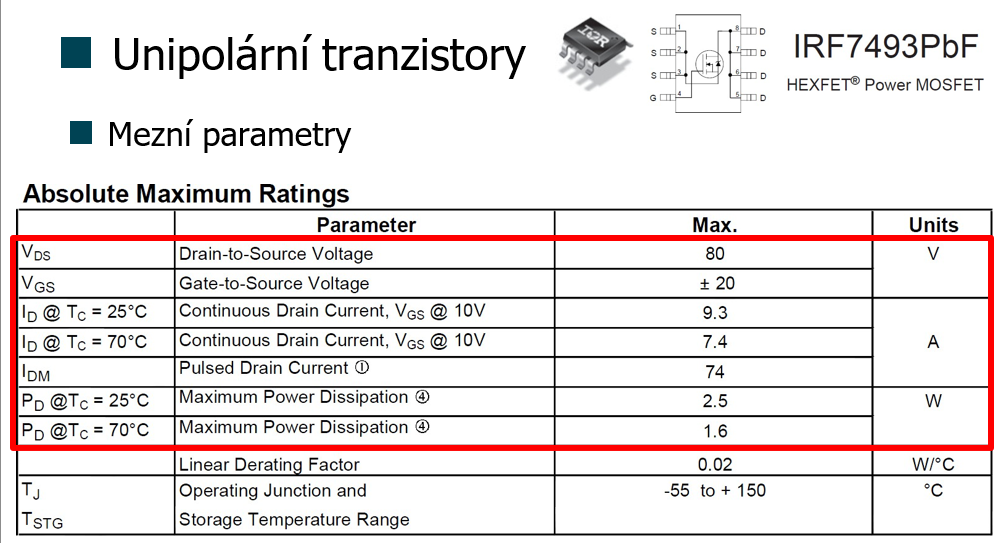
\includegraphics[width=0.65\textwidth]{img_08_mosfet_parametry.png}
  \caption{MOSFET -- parametre z katalógu, SOA charakteristika (Prednáška 8, Slide 37)}
  \label{fig:mosfet}
\end{figure}

\textbf{Výhody MOSFET oproti BJT:} napäťové riadenie (malý budiaci výkon), rýchle spínanie (žiadna akumulácia minoritných nosičov), paralelné zapojenie bez vyrovnávacích odporov.

\section{IGBT -- pre veľké výkony a napätia}

IGBT kombinuje napäťové riadenie (Gate ako u MOSFET) s malým saturačným napätím bipolárneho tranzistora pri veľkých prúdoch. Vhodný pre napätia nad 600~V a výkony od stoviek W po MW.

\begin{figure}[H]
  \centering
  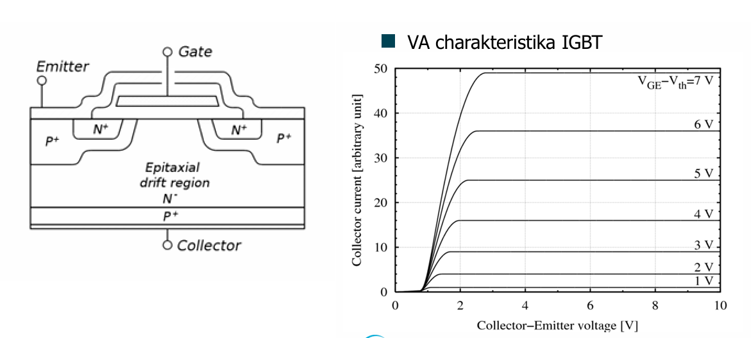
\includegraphics[width=0.60\textwidth]{img_08_igbt_schema.png}
  \caption{IGBT -- vnútorná štruktúra (MOS + bipolárny tranzistor) a VA charakteristika (Prednáška 8, Slide 48 a 49)}
  \label{fig:igbt}
\end{figure}




Nevýhoda: pri vypínaní má \textbf{prúdový chvost} (tail current) -- rekombinácia minority carriers spomaľuje vypnutie, čo obmedzuje maximálnu frekvenciu na $\approx 100$~kHz a spôsobuje vypínacie straty.

\section{Prechodové javy pri spínaní induktívnych záťaží}

\textbf{Základný problém:} indukčnosť (tlumivka, transformátor) si ``pamätá'' prúd -- pri vypnutí tranzistora chce prúd ďalej tiecť. Keďže cesta je prerušená, indukčnosť vyvolá \textbf{napäťovú špičku}:
\[ u_L = L \frac{di}{dt} \]
Pri rýchlom vypnutí môže špička niekoľkonásobne presiahnuť napájacie napätie a zničiť tranzistor.

\textbf{Straty pri spínaní} vznikajú počas prechodu cez aktívnu oblasť -- krátky okamih, keď sú na tranzistore súčasne veľké napätie aj prúd. Celkové spínacie straty:
\[ P_{sw} = (E_{on} + E_{off}) \cdot f \]
Čím vyššia frekvencia, tým väčší podiel celkových strát tvoria spínacie straty.

\begin{figure}[H]
  \centering
  \begin{subfigure}{0.48\textwidth}
    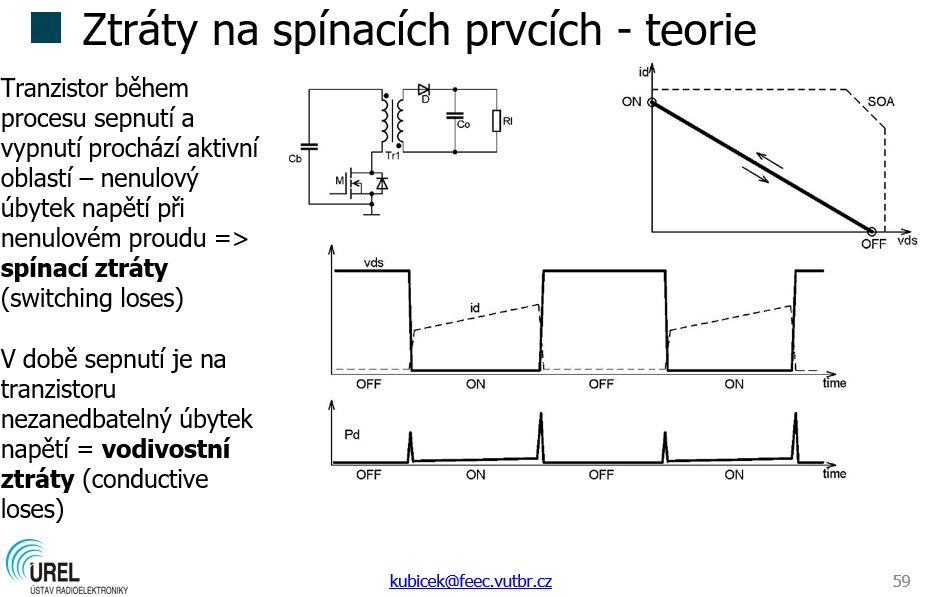
\includegraphics[width=\textwidth]{img_08_spinaci_prechodove.png}
    \caption{Idealizovaný priebeh (teória)}
  \end{subfigure}
  \hfill
  \begin{subfigure}{0.48\textwidth}
    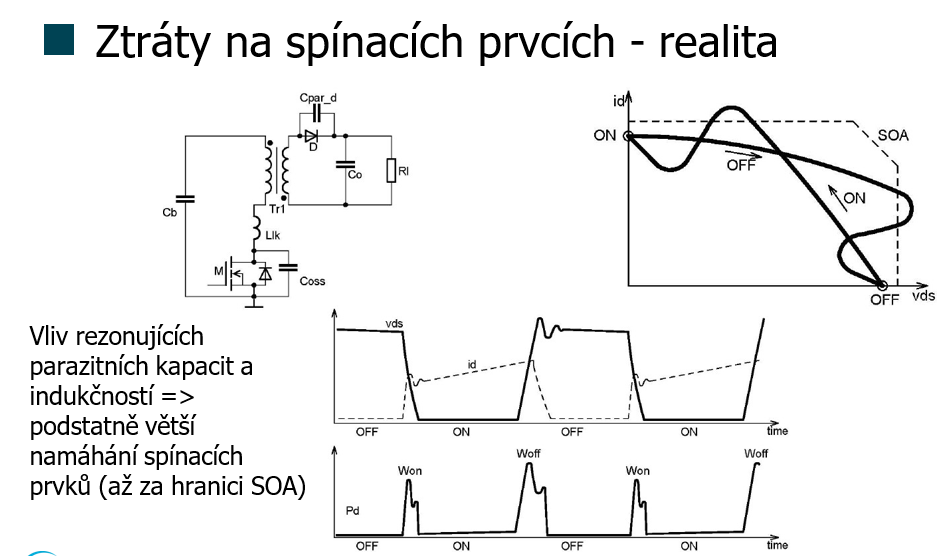
\includegraphics[width=\textwidth]{img_08_spinaci_prechodove_realita.png}
    \caption{Reálny priebeh s parazitmi}
  \end{subfigure}
  \caption{Straty na spínacích prvcích (Prednáška 8, Slide 59 a 60)}
  \label{fig:spinacie_priechod}
\end{figure}

\section{Potlačenie prechodových dejov}

\subsection{Snubbery (tlmiče)}

\textbf{Snubber} je RC alebo RCD obvod paralelne k tranzistoru alebo dióde. Spomaľuje nárast napätia pri vypínaní -- špičky sú menšie, tranzistor je menej namáhaný. Energia sa uloží do kondenzátora snubberu a v odpore sa disipuje (=straty).

\begin{figure}[H]
  \centering
  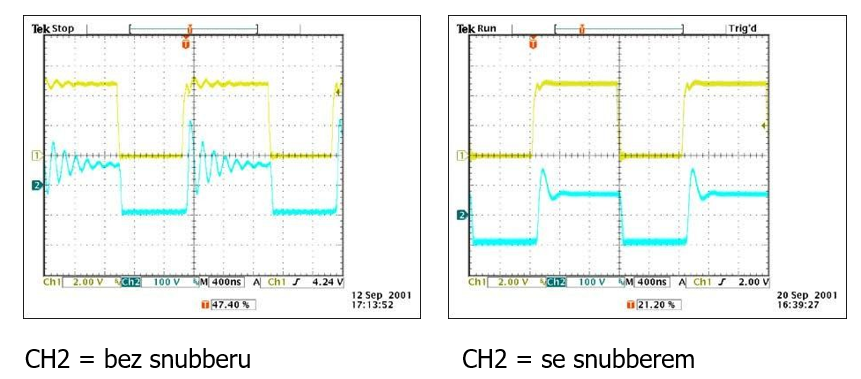
\includegraphics[width=0.65\textwidth]{img_08_snubber.png}
  \caption{RCD snubber -- priebeh napätia bez a so snubberom (Prednáška 8, Slide 63)}
  \label{fig:snubber}
\end{figure}

\subsection{Kvazirezonančné a rezonančné meniče}

Namiesto disipácie energie v snubberi možno zaradiť malú indukčnosť a kapacitu tak, aby napätie na tranzistore pred zapnutím prirodzene kleslo na minimum -- \textbf{ZVS (Zero Voltage Switching)}. Alebo aby prúd pred vypnutím klesal na nulu -- \textbf{ZCS (Zero Current Switching)}.

\begin{itemize}
    \item \textbf{Valley switching} (kvazirezonančný Flyback) -- sepnutie v okamihu minima rezonančného kmitu napätia $U_{DS}$. Jednoduché, premenná frekvencia.
    \item \textbf{LLC rezonančný menič} -- L a C v rezonančnom obvode, ZVS pre celý rozsah záťaže. Bežný v moderných PC zdrojoch a nabíjačkách notebookov.
\end{itemize}

\begin{figure}[H]
  \centering
  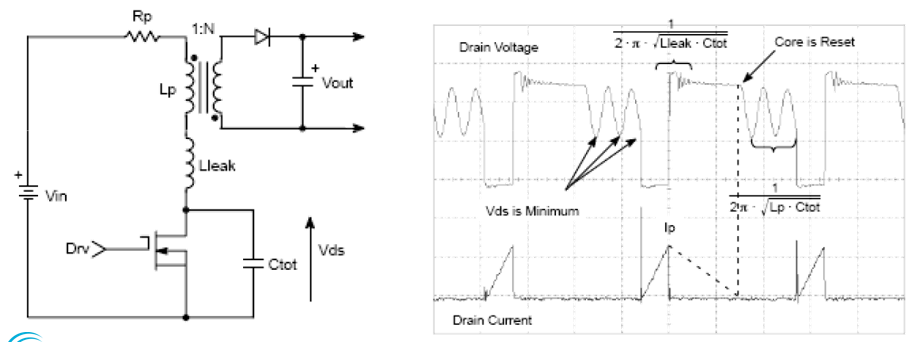
\includegraphics[width=0.65\textwidth]{img_08_kvazirezonancni.png}
  \caption{Kvazirezonančný Flyback -- spnutie v okamihu minima (valley) napätia $U_{DS}$ (Prednáška 8, Slide 65)}
  \label{fig:kvazirezonancni}
\end{figure}

\textbf{Výhody:} vyššia účinnosť, možnosť vyššej spínacej frekvencie ($\to$ menšie súčiastky), menej EMI. \textbf{Nevýhody:} premenná pracovná frekvencia, zložitejší návrh a regulácia.
